\documentclass[12pt, letterpaper]{article}
\usepackage[utf8]{inputenc}
\usepackage{mathptmx}
\usepackage{geometry}
\usepackage{siunitx}
\usepackage{appendix}
\usepackage{pdfpages}
\usepackage{amsmath, amsthm, amssymb}
\usepackage{minted}
\usepackage{hyperref}
\usepackage{xurl}
\usepackage{tabularx}
\usepackage{rotating}
\usepackage{longtable}
\usepackage{chngcntr}
\usepackage{indentfirst}
\usepackage{booktabs}
\geometry{a4paper, margin=1in}

\usepackage{graphicx}
\usepackage{setspace}
\doublespacing

\usepackage[style=apa, backend=biber, sortcites=true, sorting=nyt]{biblatex}
\addbibresource{references.bib}
\usepackage{titlesec}
\usepackage{fancyhdr}
\pagestyle{fancy}
\fancyhead[L]{Uncovering Drivers of EU Carbon Futures with Bayesian Networks} 
\fancyhead[R]{\thepage} 
\fancyfoot{} % Clear all footer settings
\renewcommand{\headrulewidth}{0pt}

\begin{document}

\begin{titlepage}
    \centering
    \Large\textbf{IE University}\\[0.5cm]
    \large\textit{School of Science \& Technology}\\[1.5cm] 
    
\includegraphics[width=0.4\textwidth]{graphics/SST.png}\\ 
    \Huge\textbf{Uncovering Drivers of EU Carbon Futures with Bayesian Networks}\\[0.5cm] 
    \Large\textbf{Jan Maciejowski}\\ 
    \large\textit{Bachelor of Data and Business Analytics}\\[0.5cm] 
    \Large\textit{Supervised by:}\\
    \Large\textbf{Prof. Manuele Leonelli}\\
    \large 30.04.2025 \\[1cm] 
\end{titlepage}

\begin{abstract}
The EUs Emissions Trading System (ETS) is an important mechanism responsible for forcing greenhouse gas emission cuts towards a net zero economy. A tradeable carbon credit, namely the European Union Allowance (EUA), is issued to be held and traded by compliant parties with large sectorial emissions. The objective of this research is to identify and estimate the effect of external variables on the price of the EUA futures. With the use of various machine-learning techniques, this work establishes a discrete Bayesian network of interdependent connections to better understand the spillage of effects to our target variable. We extend it by adding a time influence component, thus creating a dynamic Bayesian network. We use daily price data, spanning the last two phases of the ETS (2013-now), including various assets such as commodities, equity indexes, currency pairs, amongst others. Results show that the energy markets and energy commodities influence the carbon allowance demand dynamics the strongest. The heightened activity of the energy sector is heavily influenced by the performance and risk sentiments ruling the equity markets. As found, with projected disturbances to the European economy, implying higher risk, drops the energy demand and likewise the price of EUAs. Corresponding models, along with their findings, allow for compliant parties, other investors and regulators to better understand and forecast the market dynamics surrounding the EUA futures. 
\end{abstract}

Keywords: \textit{Cap and Trade, Carbon Trading, Dynamic Bayesian Networks, Energy}

\newpage

\tableofcontents

\newpage

\pagestyle{fancy} 

\section{Introduction}

The EU Emissions Trading System (ETS) is a cap-and-trade mechanism, designed to combat and lower carbon emissions within the European Union, recently updated with the approval of the Fit For 55 package \parencite{ec_ets}. Each eligible sector defined as highly emissive must comply with it by acquiring enough European Union Allowances (EUAs), matching their carbon emissions into atmosphere. One EUA makes it possible to emit one tonne of CO2. If the quantity of banked EUAs does not match the amount of emitted carbon in tonnes before the end the EUA surrendering date, the regulatory requirement is not met. In such situation, heavy fines are placed on non-compliant parties, with the obligation to acquire missing EUAs in the following regulatory period.

The EUA instrument is first auctioned in a predetermined number lowering every year, by individual countries participating in the EU ETS. The list of participants consists of all countries of the European Union, Iceland, Norway, Lichtenstein and the energy sector of Northern Ireland. Allowances are mostly listed on the German European Energy Exchange (EEX) for primary exchange. EUAs gathered above the surrendered threshold can stay with a firm to be used in the next period or can be traded on the secondary market, which mostly happens with the use of financial derivatives. This research will focus on futures contracts as they are the most traded and liquid instruments of the broad market \parencite{esma2024}. Such contracts allow for hedging EUA price risk with exchange happening at a predetermined date, mostly in December, as it is the end of compliance year \parencite{esma2024}. Certain industries at risk of carbon leakage are given several free EUAs to mitigate the risk of such sectors fleeing to countries with less restrictive regulation. However, their number is also being reduced with time. 

As the ETS directly affects the prices of energy or production costs, it has been a topic of vast political discussion within the European Union. The proceeds allocated into funds from the primary sales of EUAs are intended to support a transformation into a clean economy, especially in the energy sector. Subsequently, the effects of the ETS prices are often carried over on energy consumers, as reflected in surging electricity prices in some member states with highly emissive energy structures. These prices are often additionally amplified by unstable gas and coal prices.

The study of determinants affecting the EUA pricing is important due to several reasons. The ETS is an indirect form of carbon taxation, therefore the inflows to EU and member state budgets should be monitored along with the use of those proceeds. Collected funds should be designated with a purpose to help and invest in sustainable energy grid transformation efforts. A vast majority of the emissive sectors needs to surrender a designated number of allowances of which the price fluctuates. Such sectors are energy, heat, petroleum and associated product production, amongst other. Many financial institutions participate in trade as well. The determination of most key factors is important as such participating parties need to forecast, hedge against price risks or take profit on the broad EUA market. Understanding of those causes provides a competitive edge on the market and allows participants to anticipate future trends, and risks associated with trading of carbon credits, as such could cause price volatility or make the system ineffective.

A variety of existing research tries to analyse the major market and non-market price determinants using various statistical approaches. The purpose of this work is to enrich the current research conducted on the topic, by improving certain unaddressed problems and modelling the influence of certain factors like commodity prices and economic conditions on the price of the allowances themselves, with the use of both the Bayesian network and the earlier unused in the topic - dynamic Bayesian network (DBNs). Bayesian networks are well suited for our case of modelling financial dependencies, as they offer “a compact probabilistic representation of the system” \parencite{kitson2023}. The presented problem, to anticipate next day prices, requires capturing of time varying dependencies. This is not possible to achieve with the unmodified Bayesian network as dependencies are captured only in the context of the same day. The dynamic version of Bayesian networks is more suited for this approach as it is extended to take the concept of time into account within the model. It allows for modelling of inter-variable dependencies and influence going forward in time. This makes it a perfect fit to work with multivariate time series, allowing for a deep dive into the influence of external variables on the EUA futures in both inter- and intra-temporal dependencies, allowing for future price and risk forecasting. While many machine learning algorithms use black-box methods to try and capture predictive capabilities from data, they often are inappropriate for careful inference \parencite{kitson2023}.  We need our model to provide transparency and inform us about the importance of each variable in influence passed to the EUA futures price. The use of Bayesian networks allows for that, by addressing the chain of influence and measuring the scale of the passed effects to other nodes including the target variable. 

In the process of modelling our data, we test several machine-learning algorithms to learn both the dynamic and non-dynamic Bayesian network structures and fit the models, with the use of the “pgmpy” Python library \parencite{ankan2024}. Additionally, we use “GeNIe” for graph inference and visualization \parencite{bayesfusion}. A combination of those tools is a perfect base allowing for search of a representative network structure and discovering dependencies defying the EUA futures price.

This paper aims to contribute to current findings surrounding the list and scale of effects of external variables on the shifts in EUA futures prices. It allows for a comprehensive insight to the chain of influence surrounding the EUA, as portrayed by the dynamic and non-dynamic Bayesian networks and their changing probabilities given a certain state. The constructed graph captures complex relationships present between macroeconomic indicators, financial markets, energy sector and the EU carbon allowances pricing. We believe such presentation of the given system as a network of interdependent relations can help compliant companies covered by the ETS to prepare more informed hedging strategies. Institutional investors will have a better insight to daily price trends and regulatory bodies will be able to implement better laws protecting the European economy from abuse of secondary actors.

\pagestyle{fancy} 

\section{Literature review}

Various parties such as firms covered by the ETS, financial investors and governments need to understand the foundations behind the EUA price behaviour and its possible future implications on business operations and the overall economy, since it impacts various disciplines in Europe such as electricity prices, production costs, economic growth and others. Some factors which can be identified in the literature vary from regulatory market mechanisms \parencite{borghesi2023, tan2017}, the energy markets, including the effects of commodity markets and macroeconomic conditions \parencite{salvagnin2024, tan2017, wang2020}. In addition to that, the influence of speculation on the European carbon markets is another key subject. Next, we identify and analyse possible associations that could affect the price of the EUA futures directly and indirectly by considering five main areas. An indirect form of relationship is possible, meaning a variable can influence other variables directly linked to the ETS along the cycle. 

\subsection{Regulatory mechanisms}

As the ETS is a synthetic instrument introduced by the EU with the goal of constraining high carbon emissions with a higher operational cost, some of the most important features driving the price changes and volatility of the EUA market are regulatory mechanisms. They directly influence the supply side of the system, since the number of allowances issued for auctions is defined by their rules. Starting with what has been identified as a highly crucial element driving the change in EUA prices is the Market Stability Reserve (MSR) \parencite{borghesi2023}. It has been established in 2018, revised several times in the third and fourth phases of the ETS and made stricter with the Fit For 55 (FF55) reform.

The MSR is uniquely used in the EU, since it has no substitutes in other cap and trade solutions used around the world. Its main role was to hike up EUA prices after a vast overallocation of allowances during the first and second phases of the system \parencite{borghesi2023, salvagnin2024}. This effect was amplified by the financial crisis of 2008, when the ETS was shortly operational \parencite{borghesi2023}. 

The term Total Number of Allowances in Circulation (TNAC) is closely associated with the mechanism of the MSR. When the number of circulating EUAs is greater than 833 million, the MSR withdraws 24\% of TNAC allowances (or the difference of TNAC and the 833mln threshold) from auctions over a year, therefore decreasing the supply and increasing prices. Such process enhances system’s effectiveness in reducing carbon emissions. However, when the TNAC falls below 400 million allowances, the MSR releases 100 million new allowances in auctions, coming from its reserve. As revised with the FF55 package, the MSR holds a threshold of 400 million allowances, and all the EUAs held above this number will be invalidated for future use. The ETS has seen a rapid removal of an EUA surplus in recent years, therefore driving the price up significantly since the MSR has been introduced. 

Another aspect affecting the ETS supply is the rapidly declining emissions cap which directly translates into the number of maximum EUAs issued \parencite{ec_ets}. A yearly reduction rate known as the Linear Reduction Factor prior to the FF55 reform was set at 2.2\%. It has nearly doubled to equal 4.3\% currently, to ensure alignment to the EU’s commitment for 55\% greenhouse gas reduction by 2030 when compared to 1990 levels. The cap for 2024 equalled 1.3 billion allowances, including 57\% of it being designated for auctioning and 43\% for free allocation \parencite{ec_ets}. 

Policy parameters, including the MSR, influence market liquidity through supply-side decisions, making them extremely important elements in EUA price determination, as they affect the availability of allowances for the current and future use. Various academic institutions, carbon market analysts and financial companies (incl. BloombergNEF and Refinitiv) model their own simulation of the MSR and define it as a major factor in deciding the future price of EUA futures \parencite{ariadne2022}.

MSR and Linear Reduction Factor cause the EUA price to increase by implicating allowance cancellations and stricter reduction paths. However, the price remains highly volatile because of the firms’ behaviour in managing EUA banks for the future use. In their review of the ETS, \textcite{borghesi2023}, discuss the MSRs implications on EUA price instability. According to them, carbon allowance banks can be affected by various considerations such as economic shocks, emissions cap trajectory changes and future overlapping regulations. Furthermore, when it comes to the influence of the MSR on price volatility, even though it was made to ensure price stability by balancing supply and demand sides, the effectiveness of the ETS can be questioned. As shown by the review, the mechanism can increase volatility since it shortens the time during which companies can save EUAs for future use, therefore limiting their hedging capabilities.

Another vague point in the MSR’s use is its part in providing EUA price resilience to economic and regulatory shocks. As argued in the earlier mentioned ETS review, the MSR’s response can differ depending on the time of shock occurrence and structure. The MSR was created as a supply-restricting mechanism that removes the surplus of allowances from the broad market. No matter the direction of the future demand, the MSR ensures prices remain high, rather than responsive, to counter the effects of market shocks. For instance, as shown by the COVID-19 pandemic, the MSR absorbed a short-term lower demand shock in an efficient way. However, if such shock events affect the demand in the long term, the MSR might not be as effective in stabilising prices, due to uncertainty of the future cap levels \parencite{borghesi2023}. Additionally, regulatory changes concerning emission and coal usage laws could directly affect the market, increasing costs of production and influencing the EUA demand \parencite{salvagnin2024}.

\subsection{Commodity markets}

The price of the ETS is influenced by certain market factors like the prices of energy commodities, including natural gas, coal and oil. That is due to a direct relation of these resources, especially natural gas and coal, as main fuels used in a typical European energy mix. The phenomenon of fuel switching is an important part of influence to the EUA \parencite{lovcha2021}. Such process is defined by the change of base fuel for powerplants due to certain reasons, including price of the underlying commodities to be used. Supported by inference from a Structural Vector Autoregression (SVAR) model, EUA price movements are reflected by the significant connection to coal and natural gas \parencite{lovcha2021}. This view is supported by \textcite{tan2017} using a quantile regression model, they find a negative relationship between these commodities and the EUA price. When prices of natural gas are high, many energy production outputs switch to coal instead, which is cheaper but much more emissive, changing the demand for EUAs and influencing the price. The opposite applies for coal prices: the higher they are, the higher incentive to use the less emissive natural gas is \parencite{lovcha2021, tan2017}. Energy commodities explain most of the EUA price fluctuation as they are closely related to the ETS, however the importance of each commodity in determining the EUA price changes depending on period \parencite{lovcha2021}. Furthermore, research findings using a greedy selection algorithm applied to Information Imbalance analysis, have shown coal and natural gas prices to be highly informative in the prediction of EUA prices, as Europe’s energy sector is highly reliant on these resources \parencite{salvagnin2024}.

A third factor - oil prices – is another important element for EUA price determination. Oil has been a good predictor of natural gas prices due to two reasons. Many currently traded natural gas contracts are linked to the oil price. Moreover, oil represents an important indicator of the condition of the world economy and energy system, as it is the most traded commodity \parencite{lovcha2021}.  Again, as found with the use of the SVAR model, oil price shocks directly influence the EUA prices to soar \parencite{lovcha2021}. Additionally, the energy market directly has a positive influence on the stock market, where the S\&P 500 index is closely connected to oil prices and indirectly affects the carbon allowances market \parencite{wang2020}. 

Supply and demand volatility in oil markets are linked to the rising prices of allowances. However, higher risk volatility on oil markets reduces the price of such allowances \parencite{zheng2021}. Such oil price shocks are seen to be stronger, depending on the bearish to bullish state of the current market. The first reason explaining the relation between positive supply and demand shocks is that the latter can cause lower oil prices, which is a direct incentive for certain production sectors to use it on a larger scale, therefore increasing the demand for EUAs. On the other hand, oil risk shocks are considered a good reflector of the state of the market, as they directly affect the related oil-company equity market \parencite{zheng2021}. Such dependency is explained by rising risk and uncertainty, which pushes investors to demand higher compensation, meaning higher yields \parencite{tan2017}. Since this may affect the sectors financials and production capabilities, the lower demand for EUAs can also impact the price \parencite{zheng2021}. 

\subsection{Energy markets}

The energy sector is the biggest contributor to verified emissions within the ETS \parencite{eea}, meaning the factors affecting its performance have a relatively large influence on the carbon allowance market. On the other hand, "energy, which is the driving force of economic development and has an inseparable relationship with the financial markets, may be influenced by the fluctuation in macroeconomic risk factors \parencite{tan2017}. Fundamentally, electricity prices are an effect of two inputs – carbon permits and fossil fuels. Therefore, electricity prices are affected by the EUA prices. Theoretically, this relationship does not take place in opposite direction. However, a spillover effect of electricity prices can still affect the EUA market in a limited scope \parencite{lovcha2021}.

Electricity prices can affect the patterns in energy consumption and therefore directly influence the production costs and the economy. Following this understanding, the carbon emission traits and EUA price movements can be affected by these features. Electricity prices do play an indirect importance in determining the EUA price, often by influencing microeconomic risk. This can happen through the electricity price effect on either stronger or weaker industrial production.  The intensity of such production can also shift due to economic propulsion or fuel switching, making the energy prices more expensive. These determinants shift the associated demand for emission certificates, therefore affecting the EUA price \parencite{tan2017}. Several interdependent factors on the energy markets can cause change to both economic conditions and the EUA market.

The rising share of clean energy sources in the overall European energy mix, decreases the need for this sector to acquire EUAs. The development of clean energy technologies and their implementation therefore can directly affect the price of the ETS. This influences the demand and forces a change to the landscape of main determinants of the carbon allowance prices \parencite{salvagnin2024}. One way to evaluate the European renewable sectors’ rising importance is by measuring its equity aggregated in relevant indices. For example, ERIX index, composed of European companies within the renewable/clean energy sector, is the most informative variable in explanation of EUA price movements \parencite{salvagnin2024}. Importantly, the behaviour of the ERIX index exhibits close relationship to the behaviour of the EUA itself, since with the rising contribution of renewable sources in the energy mix, the associated emissions are being reduced \parencite{hailemariam2022, salvagnin2024}.

Following the findings from a Bayesian network model, the clean energy sector has a positive impact on the overall performance of whole energy market \parencite{wang2020}. Effects of this influence boost the stock market and economic activity, indirectly pushing EUA prices upwards with rising demand. Innovation within the energy sector, especially renewable sources, can push electricity generation to be more efficient, therefore positively affecting the equity market, which can result in lower production costs and increased economic activity \parencite{wang2020}.

\textcite{pena2022}, with the use of multiple regression models and Monte Carlo simulation, show that the rise of generation from renewable sources is highly associated with lower electricity wholesale prices. The benefits of reduced energy production costs are not transferred to household prices due to non-energy associated costs which include taxes and other levies. A paradox arises, as lower wholesale electricity costs can encourage increased economic activity and higher electricity consumption, which opposes the EU’s broad goal of carbon emissions reduction.

The EU’s carbon allowance market is a significant net spillover receiver, short and long term, from various clean energy indices \parencite{hanif2021}. According to findings from a combination of a time scale spillover index and a series of different copula functions, such an effect can be seen mainly from S\&P Global Clean Energy Index (30 globally most influential clean energy stocks) and the NYSE Bloomberg Global WIND Index (companies involved in wind turbine derived energy) \parencite{hanif2021}. This, again, signals the relevance of the clean energy sector, its development and implementation into the energy mix to the changing price dynamics of the EUA futures \parencite{hanif2021}. 

\subsection{European economic conditions}

Some further key components affecting the carbon market can be broken into several macroeconomic factors, including the commodity, stock, bond and the FX markets \parencite{wang2020}. Consistent with inference from a frequency-domain analysis, there is a connection between EUA pricing and national stock indexes, as well as the economic cycle \parencite{lovcha2021}. Shocks to economic activity are represented in response to the carbon price, especially in the third and fourth phases of the ETS. Economic growth translates into more intensive production efforts which influence the demand and therefore the price of carbon allowances \parencite{lovcha2021}. Eurozone government bond yields provide valuable information about market expectations regarding the future shape of economy. The rapid change of those expectations can cause fundamental EUA demand and price shifts \parencite{salvagnin2024}. Dynamically changing macroeconomic risk factors can strongly influence volatile behaviour in EUA pricing, where unfavourable economic conditions may lead to increased cost of money \parencite{tan2017}. Modelling of currency pairs and stock market indexes provides information accounting for changes to the global risk sentiment. As pointed out, excessive uncertainty or speculative behaviour might lead to volatility in EUA pricing \parencite{salvagnin2024}. Junk bonds can also be used to assess the hike in perceived economic risk, as they portray the yield difference between higher and lower risk rated corporates. Investors view them “as a strong predictor of stock market returns and a proxy of default risk” \parencite{tan2017}.

 The set of variables influencing the EUA price changes depending on period and economic cycle. It is also subject to change due to unforeseen events that drastically shift the current conditions surrounding the carbon allowances \parencite{salvagnin2024}. As an example, in between the third and fourth phases of the ETS the fundamental EUA price determinants have updated to ones more driven by the financial markets. This was likely stimulated by the Covid-19 pandemic, in addition to the energy crisis caused by the Russo-Ukrainian war, which heavily influenced the EUA market, signalling changing economic conditions \parencite{salvagnin2024}.
 
The influence of green and ordinary bonds on the EUA market is relatively large as these types of bonds can provide information regarding the state of the economy and the associated perceived risk measures. Green bonds are also seen as a direct way of investment into green projects, which actively work towards decreasing the emission of greenhouse gasses into the atmosphere and therefore can affect the demand on EUA markets \parencite{leitao2021}. \textcite{leitao2021} using a Markov switching econometric model, find that the S\&P Green Bond index has a positive and significant effect, both in low and high volatility ranges, on the EUA pricing in the short-term. In a different model, the Sol Green index is found to have a positive price impact in both the short- and long-term ranges. This contradicts prior research which states that the bigger the demand for renewable energy is, the less important the traditional fossil fuel-based energy market is, implying a smaller demand for carbon allowances \parencite{koch2014, leitao2021}. This can be due to rising speculation around the EUAs, as their purpose is to penalise carbon emitters more heavily with time and incentivise companies to reduce their emissions. According to findings of the same paper, another explanation for the positive relationship between Green Bonds and EUAs could be the costs of energy sources switching to renewables. As these become more important, power plants prolong the usage of fossil fuels and therefore create more demand for EUAs, which doesn’t align with the objectives of the ETS.

According to the same study, conventional bond market (with the rise of bond prices, decreasing yields) has a negative effect on EUAs; however, this result is only statistically significant in highly volatile market conditions. This contradicts prior research where in a situation of high uncertainty, investors demanded higher yields. Lower conventional bond prices (high yields) are believed to drive the EUA price downwards, as they can cause decreased borrowing due to high financing costs. This directly translates into constrained production capabilities \parencite{tan2017}.

\subsection{Role of Speculation}

The extent of speculations’ influence on the pricing and volatility of the ETS has been a matter of vast discussion amongst the political spheres of the European Union. The level of speculation is often seen as large enough to undermine the true value of the EUA itself. This topic is even more important given the EUA is an input element for the price of electricity \parencite{lovcha2021}. Furthermore, according to the Independent Commodity Intelligence Services \parencite{icis2020}, the EUA market is a perfect environment for speculation due to its high-level standardisation, high liquidity, small transaction costs and, most importantly, high volatility.

While the level of speculation is debated by many sources, a special institution, European Securities and Markets Authority (ESMA), is tasked with the oversight, reporting and enforcing regulation on the lawful trading of EUAs ever since they were classified as a financial instrument. 97\% of the secondary market exchange happens on the Intercontinental Exchange (ICE), according to \textcite{icis2020}. When it comes to the auction of allowances, 90\% of them are acquired by 10 actors from the financial sector, who serve as intermediaries \parencite{esma2024}. This signals that ETS operators prefer to source EUAs from them, due to cost effectiveness, offered by financial institutions and convenience and followed by often limited expertise in financial markets of compliant firms. Compliant companies typically hold long positions, whereas on the other side of the trade, there are banks and investment firms holding short positions. As much as 73\% of the secondary market volume was done by financial institutions \parencite{esma2024}. There is clear evidence of high-frequency trading on EUA markets, signalling some intermediaries do get involved into algorithmic trading. Two out of three most active buyers of EUAs were such firms and 39\% of total traded volumes were classified as trades on spreads, which are regarded to as low risk profile investments and cannot be directly linked as examples of speculative behaviour. The report also identifies buy and hold investors, whose goal is to gain profit on long term EUA price gains, however such practice has decreased when compared to the 2022 report.

The levels of speculation in the short time horizon are substantial \parencite{lovcha2021}. A majority of short-term variability can be explained by speculative behaviour. However, in the long-term, speculation plays little to no role in explaining the EUAs variability. In this case fundamental variables have a bigger weight in deciding the price of the ETS. Speculation can be a significant force to consider for actors relying on short-term positions and those who are sensitive to high-frequency changes \parencite{lovcha2021}.

There is also a visible presence of speculative bubbles on the EUA market. Supported by inference from the Phillips and Shi econometric framework test for multiple bubbles, \textcite{terranova2024} identify 7 bubbles in the span of 2017-2022, often associated with important regulatory events, meaning policy changes cause uncertainty which boosts speculative behaviour. These bubbles span on average 22 days which implies short-term high volatility, however due to the high frequency of these bubbles appearing as much as 10\% of the period regarded in the study was under volatile effects cause by excessive speculation. Such a high proportion of days under a bubble raises questions about the excessive influence of speculation of EUA pricing, undermining the effects of fundamental factors explained earlier in this review.

The corresponding review of existing research provides us with a series of possible explanations and factors likely to affect the EUA prices. The selection of important variables is important for phases of modelling and inference to explain existing dependencies found in the data. Such review allows us to merge existing knowledge into our analysis and provide insights about the network structure using expert knowledge. The glossary for previously used abbreviations and a summary of previous literature insights can be found in \textit{Appendix \ref{appendix:glossary}}.

\pagestyle{fancy}
\section{Methodology}

To investigate relationships between factors influencing the prices of the ETS, we implement two probabilistic models that attempt to capture dynamics between given variables. First part of this research concerns a standard discrete Bayesian network (BN). Secondly, supported by the structural model from the first part of this research, a dynamic Bayesian network is constructed to contain a time dependence capturing element in the model. Such a step allows us to illustrate the time-varying effects variables have on one another at the consequent time steps, broadening the knowledge about the relationships affecting the EUA futures both on the intra- and inter-time slice level. This section explains the approach to phases of preliminary data processing, modelling and detailed inference, with a goal of uncovering the graph structure and exploring the scale of influence amongst nodes.

\subsection{Data}

Deriving on the findings of past literature a collection of 19 variables has been gathered in attempt to try and model the causal relationship between them and the EUA prices. This action resulted in 20 variables included in the overall modelling and analysis stage. The plot of their price dynamic, depending on the phase of the ETS can be found in \textit{Figure \ref{fig:timegraphs}}. Used time series data spans in the third and fourth phases of the ETS, as these were the first fully functional periods. Therefore, all used variables span from 3rd of January 2013 up until the date of data gathering on the 31st of January 2025. All variables involved were downloaded using the Bloomberg Terminal to ensure data’s highest accuracy and quality. Variables can be divided into several categories: energy commodities, FX rates, stock indexes, volatility measures, bond indexes and energy/clean energy indexes. All assets in question along with their full names and Bloomberg tickers are available in \textit{Table \ref{tab:variables}}.

\begin{figure}[ht]
\centering
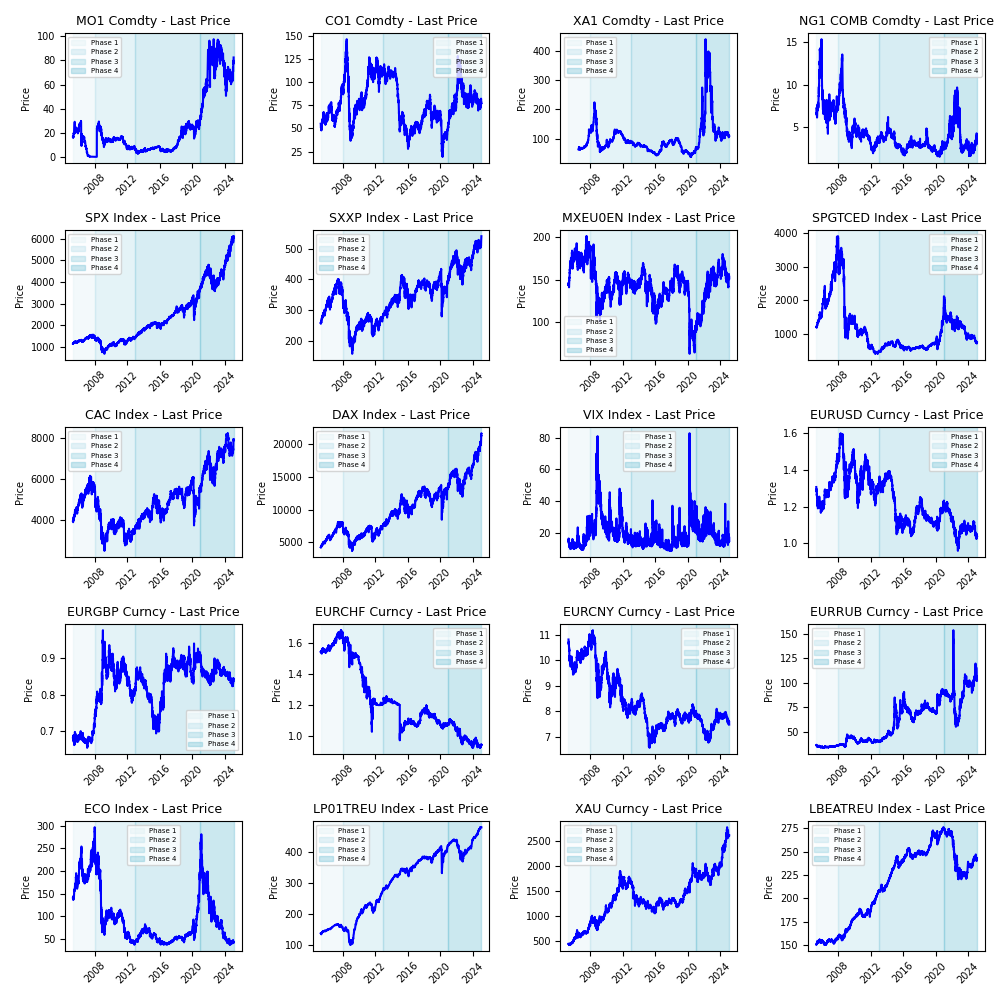
\includegraphics[width=1\textwidth]{graphics/timegraphs.png}
\caption{A time series plot of all considered factors.}
\label{fig:timegraphs}
\end{figure}

\begin{table}[ht]
\centering
\small
\resizebox{\textwidth}{!}{
\begin{tabularx}{\textwidth}{|l|X|l|}
\hline
\textbf{Category} & \textbf{Variable Name} & \textbf{Bloomberg Ticker} \\
\hline
Dependant Variable & ICE European Union Allowance Futures (1st month) & MO1 Comdty \\
\hline
Energy Commodities & ICE Brent Crude Oil Futures (1st month) & CO1 Comdty \\
{} & ICE API2 Rotterdam Coal Futures (1st month) & XA1 Comdty \\
{} & Natural Gas Futures (1st month, composite pricing) & NG1 COMB Comdty \\
\hline
Stock Indexes &	S\&P 500 Index & SPX Index \\
{} & STOXX Europe 600 Price Index & SXXP Index \\
{} & French CAC 40 & CAC Index \\
{} & German DAX & DAX Index \\
\hline
Volatility Measures & Chicago Board Options Exchange Volatility Index & VIX Index \\
{} & Gold Spot Rate & XAU Curncy \\
\hline
Energy/Clean Energy Indexes	& MSCI Europe Energy Index & MXEU0EN Index \\
{} & S\&P Global Clean Energy Index & SPGTCED Index \\
{} & WilderHill Clean Energy Index & ECO Index \\
\hline
Bond Indexes & Bloomberg Pan-European High Yield Total Return Index & LP01TREU Index \\
{} & Bloomberg EuroAgg Total Return Index Value Unhedged EUR & LBEATREU Index \\
\hline
FX Rates & Euro to U.S. Dollar Currency Exchange Rate & EURUSD Curncy \\
{} & Euro to British Pound Sterling Currency Exchange Rate & EURGBP Curncy \\
{} & Euro to Swiss Franc Currency Exchange Rate & EURCHF Curncy \\
{} & Euro to Chinese Renminbi Currency Exchange Rate & EURCNY Curncy \\
{} & Euro to Russian Ruble Currency Exchange Rate & EURRUB Curncy \\
\hline
\end{tabularx}
}
\caption{Descriptive Statistics of EUA Prices}
\label{tab:variables}
\end{table}

We include the 4 continuous futures including the target European Union Allowances (MO1 Comdty). Along with the energy commodities, we have variables directly connected to energy production such as natural gas (NG1 COMB Comdty) and coal (XA1 Comdty). These commodities act as base fuel with different emission levels, directly influencing the price of EUAs. Brent oil (CO1 Comdty) is directly related to the prices of natural gas and is a good predictor of global energy markets health. We account for these commodities as the energy sector is the biggest ETS compliance market and its state with regards to the European economic needs, is an important driver of the EUA price dynamics. The MSCI Europe Energy Index (MXEU0EN Index) tracks the performance of major European companies in the energy sector in need of EUA surrendering. Furthermore, two clean energy indexes were also included in the dataset namely the S\&P Global Clean Energy Index (SPGTCED Index) and the WilderHill Clean Energy Index (ECO Index), bringing together companies in the clean energy sector. A rapid growth in sustainable energy technologies affects the use of conventional emissive methods, therefore is an important factor for the ETS.

Various currency pairs have also been found to be an important driver in the economic cycle influencing the EUA demand behaviour. Five exchange rates to the Euro are included in our analysis including the U.S. Dollar (EURUSD Curncy), British Pound (EURGBP Curncy), Swiss Franc (EURCHF Curncy), Chinese Renminbi (EURCNY Curncy) and the Russian Ruble (EURRUB Curncy). They are an important driver to the EUA price as these economies are inter-dependent and closely tied in trade relations with the European Union. Movements in stock indexes are a good reflection of expectations regarding the state of the economy. We contain in our analysis several major including the German DAX (DAX Index), French CAC 40 (CAC Index), as they are major European indices, the STOXX Europe 600 (SXXP Index), to account for the economic shape of the whole region and S\&P 500 Index (SPX Index) to accommodate for any economic spillover effects to Europe, along with the CBOE VIX (VIX Index) illustrating future sentiments regarding market volatility.

The European bond market is another illustrator of shifts in economic risk as reflected in changing yields. The included in our dataset Bloomberg Pan-European High Yield Total Return Index (LP01TREU Index) concerns corporate non-investment grade bonds \parencite{bloomberg2021}, while the Bloomberg EuroAgg Total Return Index (LBEATREU Index) aggregates various government and corporate investment grade Euro denominated bonds \parencite{bloomberg2023}. Another measure meant to illustrate risk-off sentiments is the gold spot price (XAU Curncy) which has been proven to be a safe haven commodity in times of unknown future market conditions. Exploratory data analysis, reported in \textit{Appendix \ref{appendix:eda}}, confirms standard behaviour of financial logarithm return data, exhibiting low amounts of auto-correlation, non-normal distributions and fatter tails. The correlation matrix exhibits strong correlation between equity market indices, while the oil futures exhibit a positive relation with the European energy sector.

The code used in the process of this analysis, along with saved Bayesian network models and graphs, for experiment replication is available at: \url{https://github.com/Majon911/CapstoneETSPublic}.

\subsection{Data pre-processing}

Missing values have been filled with prior day prices, as in most cases the markets were simply closed on selected days whereas in other exchanges they were actively traded. The prices of the underlying assets and indices, behaviour typical of financial data, vary in scale. To combat this effect and normalise all variables to the same scale, daily logarithm returns have been applied.

Since this research focuses on continuous time series, there is a time dependency behaviour in the data which needs to be modelled, accounted for and removed. For our non-dynamic Bayesian network we should consider only pure non-time-dependant influence, variables have on each other. To remove the effect of such time dependence, we use an AR-Garch model, as commonly used in financial time series modelling (e.g., \cite{ruppert2015}). Frist to capture, using the autoregressive (AR) mean model, the autocorrelative behaviour in our variables. Secondly, for the variance model (Garch), to capture volatility clustering visible in the data. This action returns standardised residuals, which should be free of any significant autocorrelation and conditional heteroskedasticity. The $AR(lag)\text{-}GARCH(p,q)$ model used is the corresponding one, with $X_t$ being the mean model and $\sigma_t^2$ being the variance model:

\begin{equation}
X_t = \mu + \sum_{i=1}^{lag} \phi_i X_{t-i} + \epsilon_t, \quad \epsilon_t \sim T
\end{equation}

\begin{equation}
\sigma_t^2=\omega+\sum_{i=1}^{p}{\alpha_i\epsilon_{t-i}^2}+\sum_{j=1}^{q}{\beta_j\sigma_{t-j}^2}
\end{equation}

To implement such, we use the Python package “arch”, allowing for combining the Arch-Garch models with a series of different mean models. A similar approach is taken for the DBN, however in this case we remain the autocorrelative behaviour and remove the conditional heteroskedasticity using a variance model only. Each variable, according to the BIC metric, is chosen using the best-found model and their standardised residuals are used in later steps. More details about the Garch modelling stage and desired hyperparameter values, for both the dynamic and non-dynamic model, can be found in \textit{Appendix \ref{appendix:archgarch}}.

While there is a possibility of using continuous variables in the process of DAG exploration and finding the probability parameters of the Bayesian network, it is a very computationally intensive process. Additionally, inference using such models is much more difficult and complex compared to models using binned variables, as these show changes in probabilities directly associated with each category. Most implementations of Bayesian network learning algorithms do not work with continuous variables \parencite{beuzen2018, nojavan2017}, which often simply get automatically discretised. To enable simpler analysis and create a more interpretable model, we use quantile binning for each of the variables and encode their logarithmic return depending on the percentile. Values are encoded either as “High” if the value if above the 66th percentile, “Low” if below the 33rd percentile and “Neutral” if between those thresholds. This results in an unform distribution of each variable in data used to be fitted in the discrete Bayesian network and the discrete DBN. Quantile binning is used as the preferred binning method as it provides us with uniform non-informative priors \parencite{nojavan2017}, therefore we avoid the probabilities in the BN not being influenced too heavily by favoured prior distributions \parencite{beuzen2018}. Such approach allows for the model to be much more sensitive to shifts in conditional dependencies and for noticing more accurately the change in probabilities given the propagation of evidence from other nodes in the network. The binned data is used directly in the process of estimation of the networks structure.

\subsection{Discrete Bayesian network}

A Bayesian network is represented by a Directed Acyclic Graph (DAG), where each node $A$ represents a variable in the network. In our case, all variables such as a commodity price or a stock index historical pricing data is represented by a node as such. Nodes in a network are connected using only directed edges, no cycles are allowed due to properties of the joint probability distribution \parencite{bengal2008}. An edge from node $A$ to $B$, represented as $A\rightarrow B$, means that variable $A$ directly influences the probability distribution of variable $B$. In that relation $A$ is a parent of child $B$. Each node contains Conditional Probability Distributions (CPDs), that is a set of probability given a state of the parent nodes in the network \parencite{pearl2014}. For discrete variables a table representation of probabilities is used instead, known as Conditional Probability Tables (CPTs).  An example here can be the earlier mentioned relationship between nodes $A$ and $B$ where the probability of $B$ given $A$, $P(B \mid A)$ is expressed in the CPD of node $B$. Nodes not influenced by any prior evidence or without parents have a Marginal Probability Distribution, denoted as $P(A)$. The joint probability distribution of such network would incorporate all nodes representing random variables and their conditional probabilities given a parent. It can be defined as follows:

\begin{equation}
P\left(x_1,\ x_2,\ldots,\ x_{n-1},\ x_n\right)=\ \prod_{i=1}^{n}{P\left(x_i\ \right|Parents(x_i))}
\end{equation}

This equation leverages conditional independencies within the network, making it computationally feasible, especially given a high number of random variables \parencite{bengal2008}. That is important because with the rising number of variables, exponentially grows the size of the corresponding joint probability table. We can leverage this rule to extract information involving local dependencies which vastly ease up inference from such conditional probability tables.

A crucial part in the modelling process is the estimation of the shape of the network, i.e. the graph structure. Two approaches can be undertaken by either choosing an automated structure search algorithm or using expert knowledge to construct the corresponding DAG manually \parencite{kitson2023}. Various structure learning algorithms for PGMs exist and they divide into two categories: score-based and constraint-based. The first group measures the goodness of fit between the model and data while maximising a given score depending on the structure of the model in question. Major structural search algorithms include Hill Climb Search and Tabu Search – based on greedy local search, while its Tabu parameter enables a memory equation of recently visited structures in the search space \parencite{kitson2023}. Tabu is considered a fast algorithm, performing more efficiently than most of constraint and hybrid-based methods \parencite{scutari2019}. Exhaustive Search, a brute force method testing all possible variations, is unfeasible for networks of more than six nodes (as recommended in the “pgmpy” package) due to super exponential computational complexity.

Each of the score-based structure learning algorithms needs an information-theoretic scoring function used to search for the structure resulting in least error or a best fit to data \parencite{kitson2023}. There are several scores including the most popular one, BDeu from the Bayesian Dirichlet family. The BDeu score is defined as follows (Heckerman et al., as cited in \cite{kitson2023}):

\begin{equation}
{Score}_{BDeu}\left(G:D\right)=logP\left(G\right)+\sum_{i=1}^{n}\sum_{j=1}^{q_i}\left[log\frac{\Gamma(\frac{N^\prime}{q_i})}{\Gamma(N_{ij}+\frac{N^\prime}{q_i})}+\sum_{k=1}^{r_i}{log\frac{\Gamma(N_{ijk}+\frac{N^\prime}{r_iq_i})}{\Gamma(\frac{N^\prime}{r_iq_i})}}\right]
\end{equation}

where $G$ is the Bayesian network structure, $D$ represents the used data, $n$ is the number of variables in the network, $\Gamma$ represents the Gamma function, $q_i$ is the number of parent configurations for node $X_i$, $r_i$ is such nodes number of states, $N_{ij}$ is the count of data points where node $X_i$ has the $j$-th parent configuration and $N_{ijk}$ where such node is in state $k$ given the $j$-th parent configuration. $N^\prime$ represents the Dirichlet hyperparameter, namely the equivalent sample size \parencite{kitson2023}. This measure applies a prior probability on the network structure, controlled by passing the equivalent sample size hyperparameter. A uniform distribution of prior probabilities is assigned to each of the discrete categories to avoid overfitting and zero probabilities, especially in cases of low sample size. Other scores include the well-known AIC and BIC scores, with the second one penalising model complexity to avoid overfitting. The K2 score is another well-known equivalent \parencite{kitson2023}.

Constraint-based algorithms construct a DAG depending on a series of conditional independence tests, PC is such algorithm \parencite{colombo2014}. However, they have shown to return less accurate results than tabu search for all sample sizes \parencite{scutari2019}. Lastly, we have hybrid models which combine the functionality of both score and constraint-based strategies. One such example is Max-Min Hill Climbing (MMHC), it first estimates a skeleton of a DAG using the Max-Min algorithm and later applying the score-based Hill Climb.

All the presented methods have their advantages and disadvantages, that is why testing most possible model variations is necessary to designate a structure that is most consistent with the prior expert theory described in the literature review \parencite{scutari2013}. Each score-based model has been bootstrapped and only the connections that exist in more than 50\% of the DAGs derived from the 200 different randomly bootstrapped samples are added to the final model.

Testing a variety of different search algorithms should be followed by an evidence-based selection of a best performing methods to use for final inference. That process, as shown in the survey conducted by \textcite{kitson2023}, can be complicated depending on selected evaluation method. Following that, different algorithms, trained with various datasets, represent different aims and methodologies which often cannot be compared. There is not one methodology for evaluating a network structure and conflicting observations are a possibility when trying to evaluate such. One of the most popular approaches is the use BDeu, AIC/BIC and Log-Likelihood scores and trying to derive a model which presents highest scores on all or most metrics when compared to other model variants.

Once a desired DAG is derived, the networks’ structure and the data are combined to train the Bayesian network itself and construct the corresponding CPTs. There are two major probability estimation methods available, the first one Maximum Likelihood Estimation (MLE) does not take prior probabilities into account; therefore, it can tend to overfit to data. A second one, called the Bayesian Estimator, uses a designated prior type including scores like BDeu. Depending on type of estimation and inclusion of prior probabilities the tables differ substantially, however they do capture the dynamics of variables affecting the outcome of other variables in the network.

Lastly, certain properties of the Bayesian network are derived, and we check for independencies. The “pgmpy” package allows for Bayesian network exports using the XMLBIF format. Such export allows for further exploration of the model and inference of causal relationships using “GeNIe”.

The probabilistic inference process is established as proceeded. For every variable in the Bayesian network, we provide evidence of a price change, as either “High” or “Low”. Given that evidence, the effects of nodes direct influence on each other propagate through the network to establish new probabilities of prices in different nodes of the network. That applies equally to our target variable of EUA futures, where we can directly read the change in CPTs of carbon allowance price, given the evidence in another node in the network. If computationally feasible the Bayesian network can be manipulated using functions like Variable Elimination to check for causal relationship between variables \parencite{bengal2008}. In bigger networks, the conditional probability tables grow exponentially with the number of variables, deeming it next to impossible to conduct any kind of inference. Such approach allows us to portray the effect of the nodes influence, which cause the probabilities to deviate from the uniform distribution. This allows us to assess the direction and comparative strength of the influence given to EUA. In addition to that we evaluate the equivalence classes to determine the definite directions of influence in the network. Lastly, we run sensitivity analysis implemented in “GeNIe” to assess the importance and amount of the effect from nodes in our network, transferred to our target variable of EU carbon allowances.

\subsection{Discrete dynamic Bayesian network}

The next step in our analysis is construction of an inter-temporal, 2-time-slice Bayesian network (2-TBN) in attempt to capture the possible traits of time-dependant influence variables in the network have on one another. As described by \textcite{koller2009}, a DBN is based on the concept of stationarity assumptions, meaning the dependency structure and CPDs of the resulting network do not change with time, only the evidence given to the network changes. Furthermore, Markov assumptions play another key role in this model, stating that the future state of a network can depend only on the present state of the network and not past. This blocks the possibility of nodes in $T-1$ affecting the nodes in $T+1$ and the propagation of probability changes given some evidence is only possible in consecutive timesteps evolving in a chain like manner. There are two necessary elements defining a DBN: the initial state distributions $B_0$ and a transition model $B_\rightarrow$ \parencite{koller2009}. The first element is described by the data’s prior probability and the first-tier network structure, while the transition element describes the systems evolving probabilities over time in concurrent tiers, expressed as a CPD $P(X^\prime \mid X)$, where $X^\prime$ denotes the systems state at the future time $T+1$ and $X$ at $T$. The conditional probability distribution represented by a 2-TBN is the following \parencite{koller2009}:

\begin{equation}
P\left(X^\prime\ \middle|\ X\right)=\ \prod_{i=1}^{n}{P\left(X_i^\prime\ \right|\ Parents\ X_i^\prime)}
\end{equation}

This creates two different kinds of connections between nodes of a potential 2-TBN model. Intra-time-slice between nodes at the same timestep, repeating in the same structure in every other future timestep and inter-time-slice, of edges linking nodes of a previous time slice with the nodes of the next one only \parencite{koller2009}. In other words, intra-time-slice links model the variables influence on the target variable in the span of the same timestep, in our case a day. Inter-time-step edges describe any other significant influence of a variable to the state of the same variable or a different node in the network at the next timestep, modelling the influence of prior day prices on the next day prices in the network.

An important challenge in modelling DBNs is drafting the appropriate methodology of finding the relevant structure of a network with time-dependant links. There exists no well-established method of finding the graph structure of a dynamic BN, however there is a variety of secondary approaches in search of the relevant links in between inter-temporal nodes \parencite{murphy2002}. One method used during this research is using the same structural search algorithm as for the previously trained non-dynamic discrete Bayesian network. We keep method consistent with the settings found to be the best performing in the previous part of our study, however the list of possible input edges changes.

Due to the properties of the DBN all edges leading from nodes $T+1$ back to ones in $T$ are forbidden, as it is impossible for future information to affect the distributions of nodes in the past. We blacklist all intra-time-slice connections, since they are already accounted for by the previous non-dynamic model. This allows for the search space to only include connections outgoing from nodes at $T$ to nodes in $T+1$. Such blacklist is passed to the structural search algorithm of our choice, coherent with the findings of the previous part of the research. Similarly to our approach for structure learning in non-dynamic BNs, we bootstrap the output of the algorithm incl. methods like Hill Climb, Tree Search or PC to select only the connections that are present in more that 50\% of the found structures. After that the intra-level connections from the non-dynamic BN and the inter-level links from the structural search algorithm for time dependant relations are combined to consist of a full list of edges for the purpose of DBN training to the data distributions.

After training is completed, the constructed DBN along with its time-dependant CPDs is analysed in search of significant dependencies in the model. This takes place by comparison of probabilities in EUA futures given evidence in a different node at $T=0$. The effect of such is seen by changing probabilities, deviating from uniform distribution at $T+1$. The effect and amplitude to the shift in resulting probabilities in the consecutive time steps is measured and inferred from.

\pagestyle{fancy}
\section{Results}
\subsection{Comparison of model scores with regards to various structure learning algorithms}

A series of different BN model variations were created combining the use of non-parametric bootstrap, different structure learning algorithms and adjusting of their corresponding hyperparameters. The structure search algorithms include the score-based Hill Climb, Tree Search and constraint-based PC. The corresponding algorithms were run using the “pgmpy” implementations and the Bayesian network was fitted along with the structure found by such algorithm. The resulting networks with data fitted to them using either the maximum-likelihood or Bayesian estimators were evaluated each using a set of standardised metrics such as evaluation of the performance of each of those structure learning algorithms is exhibited Loglikelihood, AIC, BIC, BDeu and K2. The selected results of the discussed methods and metrics describing selected models, incl. learned structure and parameters, goodness of fit to data is expressed in \textit{Table \ref{tab:modelscores}}.

\begin{table}[ht]
\centering
\footnotesize
\resizebox{\textwidth}{!}{
\begin{tabularx}{1.2\textwidth}{|X|X|X|X|X|X|X|X|X|X|}
\hline
\textbf{Structure\newline Learning\newline Algorithm} & \textbf{Tabu\newline Setting} & \textbf{Scoring\newline Function} & \textbf{Equivalent\newline Sample\newline Size} & \textbf{Evaluation\newline Function} & \textbf{Log-likelihood} & \textbf{AIC} & \textbf{BIC} & \textbf{BDeu} & \textbf{K2} \\
\hline
Hill Climb & 100/\newline Default & BIC & - & MLE & -59799,3 & -60011,3 & -60651,8 & -60431,8 & -60391,5 \\
Hill Climb & 100/\newline Default & AIC & - & MLE & -56659,3 & -61563,3 & -76380,8 & -74611,5 & -62271,5 \\
Tree Search & - & Chow-Liu & - & MLE & -60339,9 & -60455,9 & -60806,4 & -60706,1 & -60710,6 \\
Hill Climb & 100/\newline Default & BDeu & 1 & BE & -59877,0 & -60060,8 & -60616,8 & -60721,7 & -60407,0 \\
Hill Climb & 100/\newline Default & BDeu & 10/\newline Default & BE & -59613,3 & -59883,0 & -60704,9 & -60422,5 & -60329,6 \\
Hill Climb & 100/\newline Default & BDeu & 50 & BE & -59406,8 & -59860,7 & -61298,9 & -60426,2 & -60473,0 \\
\hline
\end{tabularx}
}
\caption{Score comparison of selected score-based structure learning algorithms}
\label{tab:modelscores}
\end{table}

By comparison of scores of the selected methods, the Hill Climb algorithm using BDeu exhibits lowest measures in four out of five rubrics. The model with an equivalent sample size of 10 is the one that has the highest Bayesian Dirichlet family scores BDeu and K2. The log-likelihood metric is the highest for the AIC driven Hill Climb model, however it lacks in different scores heavily penalising complexity including BIC and BDeu. The complexity of connections for the AIC graph is shown in \textit{Figure \ref{fig:netaic}} in \textit{Appendix \ref{appendix:graphtests}}. The Tree Search algorithm drafts measures that are worse than those of other methods, none of the metrics go above negative 60 thousand. While most of its edges were consistent with the market theory, as shown in \textit{Figure \ref{fig:nettreesearch}}, Hill Climb was found to be more coherent with the existing theory. The Hill Climb with the BIC scoring function is yet another well-performing model with good metrics along all five categories of our study. However, Hill Climb with a BDeu scoring function and an equivalent sample size of 10 exhibited better performance in scores including Loglikelihood, AIC, BDeu and K2. While comparing the networks of these two models, we can draft a conclusion that they are structurally very similar. The BIC search driven graph can be found in \textit{Figure \ref{fig:netbic}}. The BDeu method, however, drafts a small number of additional edges in comparison to the BIC scored Hill Climb, slightly increasing the model complexity.

Lastly, only computationally feasible to our purpose constraint-based method we succeeded in running is PC. As portrayed in \textit{Figure \ref{fig:netpc}}, it has 3 separate components and a very limited number of links, making it a much less complex network to those derived from score-based algorithms. Certain relationships found by the PC algorithm were found to be existent and significant in structures found by other algorithms, with the only major difference being the target variable influencing the price of coal futures. Such relationship exists in score-based models, but in the opposite direction. Hybrid models including MMHC and Hill Climb Search based on the K2 score were found infeasible to run given number of variables and edges, and drew numerous errors either in the structure discovery phase or in modelling of the probabilities within the Bayesian network itself. 

\subsection{Identifying the selected networks clusters of variables}

The selected as best performing Bayesian network fitted to data using the BDeu Bayesian Estimator showcases certain important properties affecting our target variable. Such relation is exhibited as the estimated change to probability of a price change to EU Allowances, given evidence of low, high or neutral price changes in affecting variables. As shown in \textit{Figure \ref{fig:bayesnet}} (look \textit{Appendix \ref{appendix:graphtests}}, \textit{Figure \ref{fig:netbdeu}} for Graphviz representation), the chain of influence to the target variable can be divided into certain variable subsections. Nodes of similar asset class, including for example energy commodities, stock indices or bond indices, tend to cluster together in the network. Certain nodes showcase this property including the major American stock index - S\&P 500, with direct links to the green ECO Index, associating American companies in the clean energy sector and the VIX index which directly measures volatility on S\&P 500 options. Another cluster involves European stock indices these include the STOXX Europe 600, the French CAC 40 and the German DAX. Both the American and European market clusters relate to an edge between the S\&P 500 and the STOXX 600, as well as to the CAC. The global S\&P Clean Energy Index affects the stock indices of both continents. Another cluster is constructed of nodes surrounding the European energy markets. These involve the very important MSCI Europe Energy Index in the centre, aggregating equity of major European companies in the broad energy sector. Energy commodities are amongst the ones directly affected by the previous node, such include coal and brent oil futures. Indirectly, natural gas, affected by the oil price and the EUA futures, further affected by both the MSCI Europe Energy index and coal prices, are also members of this cluster. On the border of a different cluster connecting the different exchange rates of the Euro compared to foreign national currencies and the energy cluster sets the Russian Ruble. It is affected by the European energy sector index and affects the oil prices. The U.S. Dollar plays an important role in the FX cluster, as it directly influences the rates of 3 different currencies namely the British Pound Sterling, Swiss Franc and the Russian Ruble. An outlier not belonging to any cluster is the spot gold price is also influenced by the exchange rate of the Dollar. Our last small cluster consists of two nodes, interconnected with the stock market and European energy markets, represents the bond indices. This group includes indices containing both investment and non-investment grade bonds from the Eurozone or denominated in Euros.

\begin{figure}[ht]
\centering
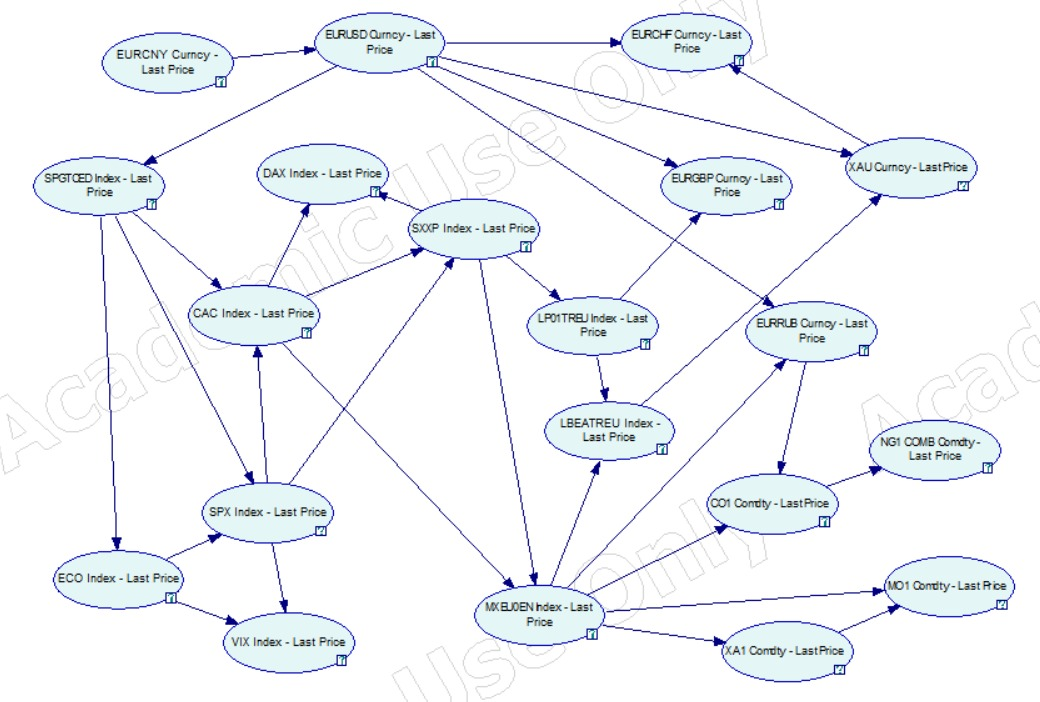
\includegraphics[width=1\textwidth]{graphics/GenieBN.jpeg}
\caption{Selected Bayesian network structure.}
\label{fig:bayesnet}
\end{figure}

\subsection{Equivalence classes of the selected models}

A partial directed acyclic graph (PDAG) was illustrated from the Genie software, illustrated in \textit{Figure \ref{fig:equlavenceclass}}, it showcases the same Bayesian network with both directed (black arrows) and undirected edges (red lines). To understand the models’ implications the concept of equivalence classes is key. An equivalence class is a set of interconnected network structures, with the same skeleton and V-structures. Given class equivalence networks share the exact same set of CPDs. This property allows for edge direction variations, that do not influence the model properties \parencite{chickering2013}. In other words, the directions between some nodes of the structure are not strictly determined by the model. As represented by the red lines, bidirectional connections mean either a circular connection between two nodes or uncertainty in direction. Black arrows mean, that if changed their direction, the statistical properties of the model would change, meaning we can infer causal relationship of one variable on the other.

\begin{figure}[ht]
\centering
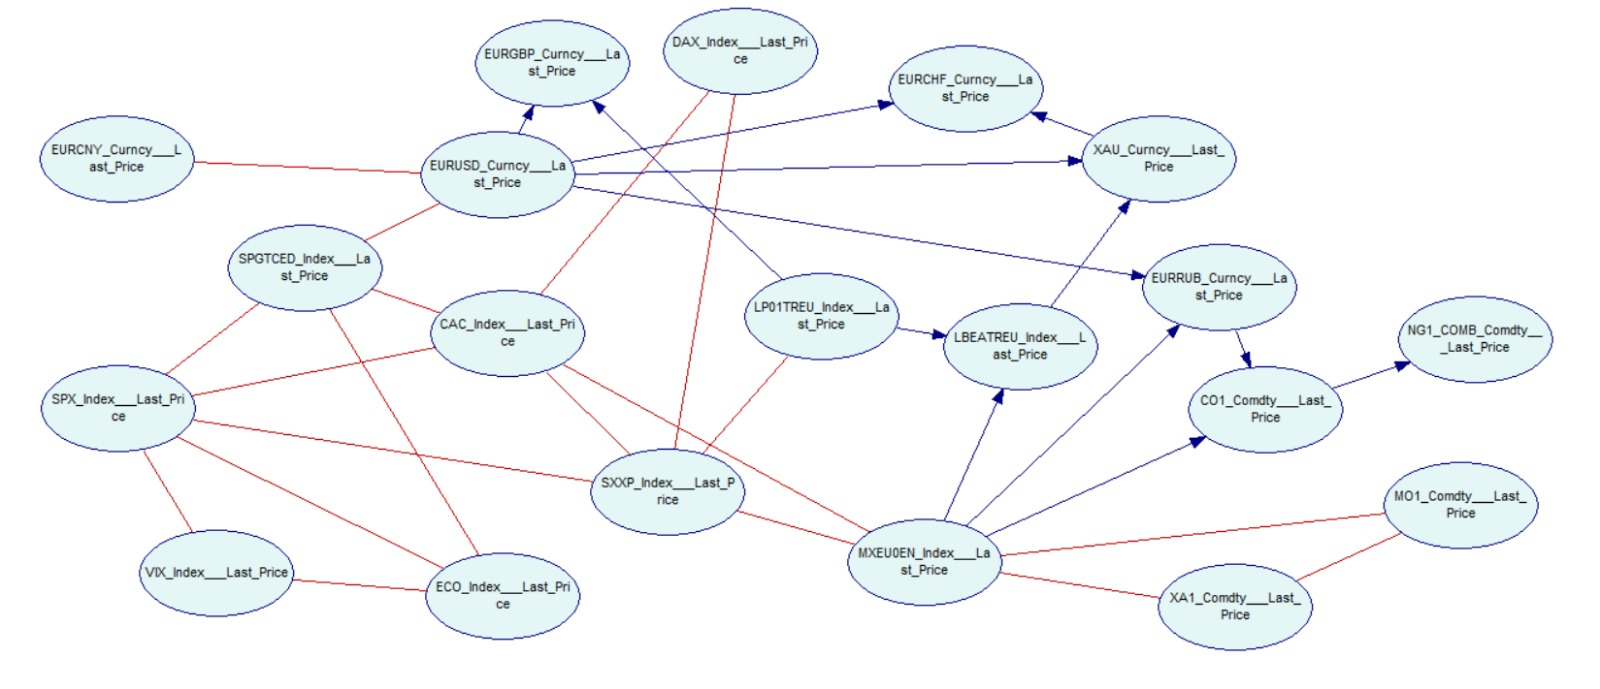
\includegraphics[width=1\textwidth]{graphics/equvalenceclass.jpeg}
\caption{Equivalence class showcase.}
\label{fig:equlavenceclass}
\end{figure}

The equivalence class showcases that no direct influence can be determined for most of the network’s connections. This property applies to nodes in various clusters mostly in the American and European stock index clusters. Link direction cannot be determined in the relation between the U.S. Dollar and the Chinese Renminbi and between the STOXX 600 index and the European high-yield bonds. More importantly, the direction of relationship between the STOXX 600 and the MSCI Europe Energy index cannot be determined as well. Finally, our direction of effects flowing between our target variable of EUA futures, the energy index and coal futures cannot be established either. The variables with established direction of influence include the European energy sector influencing investment grade bonds, the Russian Ruble exchange rate and the price of brent oil futures, which subsequently affects the natural gas futures. Further directed edges include connections originating from the U.S. Dollar which undertakes an important role in the graph. It affects directly other currencies like the Franc, Pound, Ruble and the gold price, which is also affected by the price of investment grade bonds. Two other connections are European high-yield bonds affecting the Pound exchange rate and the Ruble influencing the oil futures.

\subsection{Sensitivity analysis of effects passed to the EUA}

From the viewpoint of our target variable, the EUA price changes are highly sensitive to a select bunch of variables. As showcased in sensitivity analysis in \textit{Figure \ref{fig:sensitivity}} by the darkest shade of the red colour, the strongest relation is driven from the price of Rotterdam coal futures. This is followed by a variable influencing both the EUA and coal futures prices, which is the MSCI Europe Energy Index. It is composed of major European companies in the energy sector and its directly influenced by the European stock markets. Following this analysis the STOXX 600 is the next most significant component driving EUA price changes. The other important variables are the CAC Index, S\&P Global Clean Energy Index and the American S\&P 500, which as mentioned earlier are interconnected and with the lowest sensitivity to influence EUA price changes.

\begin{figure}[ht]
\centering
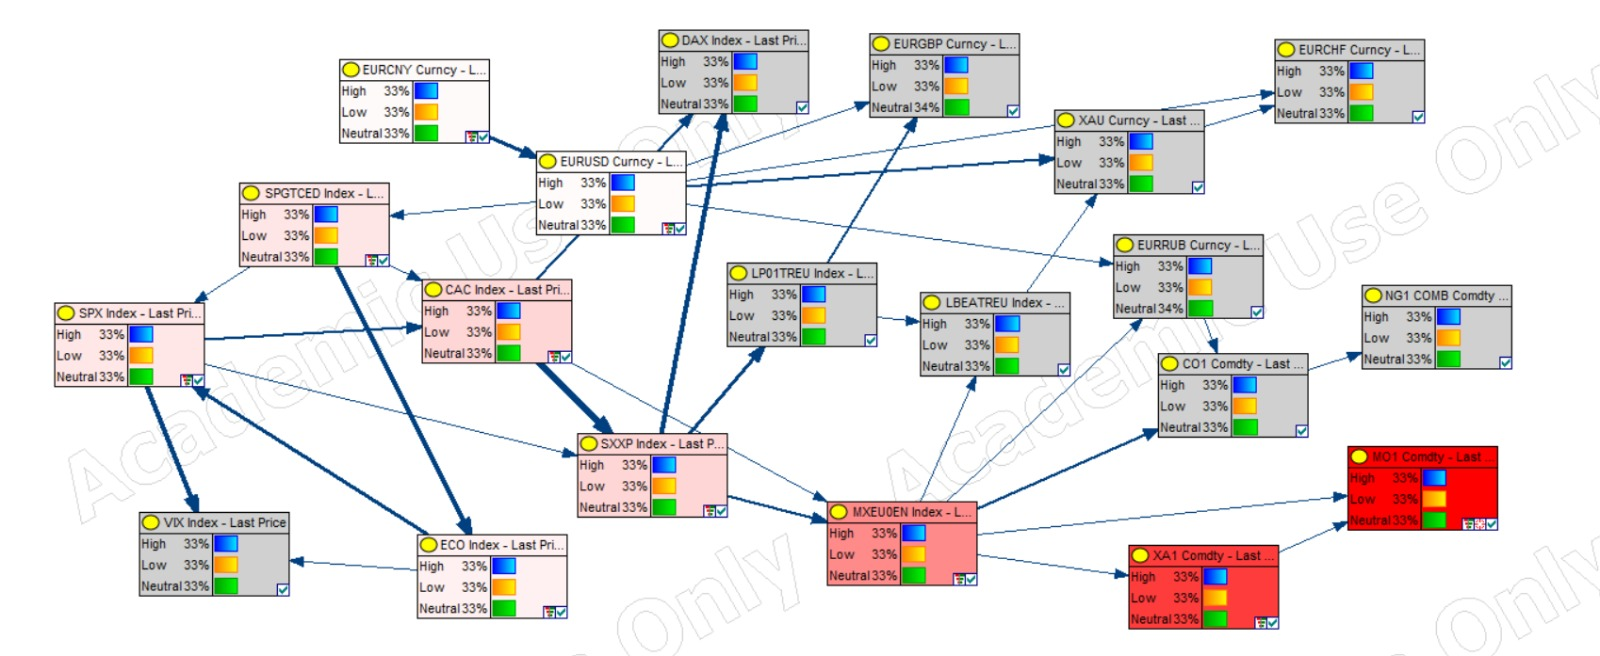
\includegraphics[width=1\textwidth]{graphics/StrengthAnalysis.jpeg}
\caption{Sensitivity analysis of factors influencing EUA prices and connection strength.}
\label{fig:sensitivity}
\end{figure}

\subsection{Results of the effects and their strength in the discrete Bayesian network with regards to the EUA}

Due to the choice of quantile binning, all nodes have a uniform probability distribution across all classes, given no passed effect from the evidence node. The results of evidence changing the probability of a EUA price return are available in \textit{Table \ref{tab:evidhigh}} and \textit{Table \ref{tab:evidlow}}, for the scenarios of a price hike or a drop, respectively. Concerning the influence of various external variables on the EUA price dynamics, as shown by the sensitivity analysis, coal futures are the biggest determinant of the EUA price regime. There exists a positive relationship between these two variables, the high return on coal future prices influences a high price of EUA. When the coal prices fall, allowance prices fall as well. The node with second most influence on our target variable is the MSCI Europe Energy Index. This index positively affects the price changes of our target variable; again, a high return on the European energy sector companies results in a higher probability of a high price shift on EUAs. A decrease in value of the index causes the highest probability of a decrease in the price of allowances. The MSCI Europe Energy index is a parent of coal futures which it also affects, shifting the relationship effect on the EUA both through coal and directly from itself.

\begin{table}[ht]
\centering
\small
%\resizebox{\textwidth}{!}{
\begin{tabular}{|c|c|c|c|}
\hline
\textbf{Node} & \textbf{High} & \textbf{Low} & \textbf{Neutral} \\
\hline
XA1 Comdty (Coal) & 43\% & 25\% & 32\% \\
MXEU0EN Index (MSCI Euro. Energy) & 40\% & 27\% & 33\% \\ 
CO1 Comdty (Brent Oil) & 36\% & 30\% & 33\% \\
NG1 COMB Comdty (Natural Gas) & 34\% & 33\% & 33\% \\
EURRUB Curncy & 32\% & 35\% & 33\% \\
SXXP Index (STOXX Euro. 600) & 37\% & 30\% & 33\% \\
DAX Index & 36\% & 30\% & 33\% \\
CAC Index & 37\% & 30\% & 33\% \\ 
LP01TREU Index (BB High-Yield Bonds) & 35\% & 32\% & 33\% \\
LBEATREU Index (BB Investment Grade) & 33\% & 34\% & 33\% \\
SPX Index (S\&P 500) & 35\% & 32\% & 33\% \\
VIX Index & 32\% & 35\% & 33\% \\
ECO Index (WilderHill) & 34\% & 32\% & 33\% \\
SPGTCED Index (S\&P Clean Energy) & 35\% & 32\% & 33\% \\
EURUSD Curncy & 34\% & 33\% & 33\% \\
EURCNY Curncy & 33\% & 33\% & 33\% \\
EURCHF Curncy & 33\% & 33\% & 33\% \\ 
EURGBP Curncy & 33\% & 34\% & 33\% \\
XAU Curncy (Gold Spot) & 33\% & 33\% & 33\% \\
\hline
\end{tabular}
%}
\caption{Change in probability of EUA (MO1 Comdty) logarithm return given evidence of a surge in value of a node.}
\label{tab:evidhigh}
\end{table}

\begin{table}[ht]
\centering
\small
%\resizebox{\textwidth}{!}{
\begin{tabular}{|c|c|c|c|}
\hline
\textbf{Node} & \textbf{High} & \textbf{Low} & \textbf{Neutral} \\
\hline
XA1 Comdty (Coal) & 25\% & 43\% & 32\% \\
MXEU0EN Index (MSCI Euro. Energy) & 27\% & 42\% & 32\% \\ 
CO1 Comdty (Brent Oil) & 31\% & 36\% & 33\% \\
NG1 COMB Comdty (Natural Gas) & 33\% & 34\% & 33\% \\
EURRUB Curncy & 35\% & 32\% & 33\% \\
SXXP Index (STOXX Euro. 600) & 30\% & 37\% & 33\% \\
DAX Index & 30\% & 37\% & 33\% \\
CAC Index & 30\% & 37\% & 33\% \\ 
LP01TREU Index (BB High-Yield Bonds) & 32\% & 35\% & 33\% \\
LBEATREU Index (BB Investment Grade) & 34\% & 33\% & 33\% \\
SPX Index (S\&P 500) & 32\% & 35\% & 33\% \\
VIX Index & 34\% & 32\% & 33\% \\
ECO Index (WilderHill) & 32\% & 35\% & 33\% \\
SPGTCED Index (S\&P Clean Energy) & 32\% & 35\% & 33\% \\
EURUSD Curncy & 33\% & 34\% & 33\% \\
EURCNY Curncy & 33\% & 33\% & 33\% \\
EURCHF Curncy & 33\% & 33\% & 33\% \\ 
EURGBP Curncy & 34\% & 33\% & 33\% \\
XAU Curncy (Gold Spot) & 33\% & 33\% & 33\% \\
\hline
\end{tabular}
%}
\caption{Change in probability of EUA (MO1 Comdty) logarithm return given evidence of a drop in value of a node.}
\label{tab:evidlow}
\end{table}

Three other contributors in the energy cluster affect the probability of an EUA price. Even though not directly influencing the parents of our target variable, oil prices exhibit a positive relationship with EUA. A high change in brent oil prices causes the probability of a high allowance price to be 3\% higher from baseline. The inverse presents a drop in EUA value. Another factor are the natural gas futures, influenced by the oil futures. However, they have a weak positive connection to the EUAs and shift the probabilities by only around 1\%. The last variable affecting the energy sector and therefore the price of EUAs is the exchange rate between the Euro and the Russian Ruble. The price of this foreign currency negatively affects the prices of EUAs, through an effect on the price of associated fuel commodities. High price change to the cost of Euro, means a drop in the price of associated energy commodities and EUAs. A cheaper Euro means a respective rise in returns on EUA futures.

Traversing downwards the chain of influence for our target variable, several stock indices were found to be significant factors. Starting with the broad European STOXX 600 it showcases a positive relationship with EUAs. A high change in price of the stock index, pushes the probability of a high change in European allowance prices. The inverse drives EUA prices down. A similar relationship can be found in the French and German indices, composites of STOXX 600. A high change to price of CAC and DAX, also causes the price of the EUAs to shift to high returns. The drop in CAC and DAX values means a higher probability of an EUA price having a negative return. As for the influence of the American stock market on the European markets and therefore the EUA prices, there is a positive relationship between the S\&P 500 and the EUA. High price changes to the shares of the biggest 500 American publicly listed companies indirectly cause an increased chance of a high change in the price of carbon allowances. Following that, a loss in S\&P 500 value is associated with a lower price of the EUA futures. The VIX Index, which behaves inversely in relation to the S\&P 500, also exhibits an insignificant negative relationship with EUA prices. A high rise in the value of the VIX Index is associated with a higher probability of a decreasing price of the EUA. A low index value rules a high price of equity on both American and European markets, causing the price of the EUA to shift higher.

Starting with the ECO Index, which considers only American companies in the green sector, there exists a small positive relationship between the hike in prices of the ECO index and the price of the EUA. When the value of the same index drops, the probability of a negative shift in EUA price increases. The S\&P Global Clean Energy Index exhibits the same positive relationship with the EUAs. Its elevated return means a greater probability of a high price change of EUA futures. A drop in index value means a higher chance of a decrease in allowance price.

The Chinese Renminbi shows a small probability change to the price of EUA (of < 1\%), neither does the Swiss Franc, nor the spot price of gold. While the probability changes for other currencies are very small, they still exist – the relationship can be described positively for the Dollar, but it is negative for the Pound, both result in a shift of 1\% to the probabilities. Gold shows a negative influence on the EUA futures price, again shifting the probabilities by just 1\%. FX pairs in relation to the Euro affect each other in a positive relation.

The last two important variables included in the analysis regard bonds, both investment and non-investment grade.  The Bloomberg High Yield Index, containing non-investment grade bonds, which require higher yields with expectations concerning rising risk, is positively related with the price of EUAs. A high value of an index price, meaning low yields on bonds is associated with a higher probability of a high price shift in carbon allowances. For low bond prices and high yields in situations of rising perceived risk and economic turndowns, the probability of a low EUA price rises. Lastly, investment grade bonds have a limited influence on the probabilities of EUA price shifts. They exhibit a negative relationship to EUA prices, with low investment grade bond prices rising the probability of a high EUA price by only 1\%.

\subsection{Results of the time-dependant effects in the dynamic Bayesian network with regards to the EUA}

The Hill Climb search algorithm with a BDeu scoring function and an ESS of 10 has drafted seventeen inter-temporal edges leading from the nodes placed within time $T$ to nodes in $T+1$. Four of these connections were self-loops connecting the same nodes in $T$ and $T+1$, showcasing significant evidence of autocorrelation at lag 1. Such a set of inter-temporal connections has been drafted towards the completion of the DBN model structure, to draft the corresponding results present in \textit{Figure \ref{fig:dbn}}.

\begin{figure}[ht]
\centering
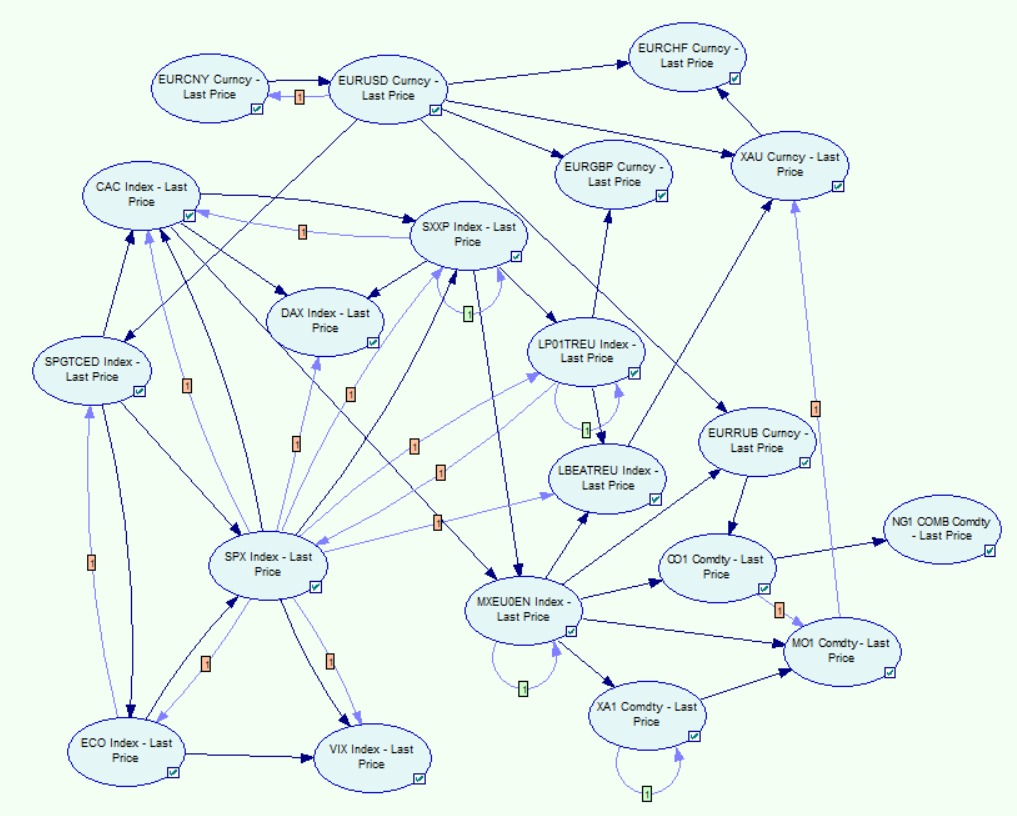
\includegraphics[width=1\textwidth]{graphics/DBN.jpeg}
\caption{Dynamic Bayesian network structure.}
\label{fig:dbn}
\end{figure}

A vast majority of the found edges are outgoing connections of the S\&P 500 Index at $T$. Such links are directed into other S\&P 500 affiliated indexes such as the American WilderHill Clean Energy index and the VIX index. More importantly to our model, European counterparts such as the STOXX Europe 600 and the German \& French CAC and DAX indices are also affected in $T+1$ by the American index in $T$, along with the European investment and non-investment grade, high yield bond indices. With a total of 7 inter-temporal edges outgoing from this major American index, we consider this variable to be very important in passing valuable information to following time slices. The effect of evidence in the S\&P 500 variable is visible in the inter-time slice connected nodes at future time steps, especially at $T+1$. The effect of this evidence decays over time, given no further evidence is provided to the model.

From other relevant connections found by the Hill Climb algorithm, the ECO Index transmits a time dependent effect to the S\&P Global Clean Energy Index, which within the intra-graph level is directly correlated with the performance of the S\&P 500. Furthermore, the U.S. Dollar influences the Chinese currency as exhibited in a $T$ to $T+1$ link.

Concerning the inter-temporal links around our carbon allowances target variable, the structural search algorithm has drafted two edges - one outgoing and one incoming. First, surprisingly, the EUA seems to have a direct time dependent influence towards the gold spot prices. Second, the EUA price shifts seem to be influenced by the prior day price shifts of Brent Oil futures.

The self-loops present in the model are the European STOXX 600 index, the non-investment grade Bloomberg High Yield bond index, as well as the MSCI Europe Energy index and the Rotterdam Coal futures. The last two are especially important to the purpose of our research as there are variables with direct intra-temporal edges to the EUA futures. Here, given future timesteps, they exhibit some change in probability distributions compared to the baseline given evidence in $T$. The strength and the direction of the effect varies depending on node. The STOXX 600 has a higher probability of a drop or small change in value the next day after a high return in $T$. Given a drop in the index value, the next day change probability is estimated to be equally a gain or a drop in the index value. All other self-looped variables follow a higher positive association, where a high rise in price at $T$ means a greater chance of a high price change next day. Similar suit follows the drop in value of an asset, which hikes up the probability of a drop happening the following day. This is especially visible for the high yield bond index and the coal future, with the effect weakening for the MSCI Europe Energy index.

The change in the next day probabilities of our target variable is often weak and close to the baseline probability of 33\% per binning category, which is an effect of the chosen quantile binning strategy. Starting with the effects of variables closest to the EUA, the oil futures rise in price in $T$ affects the probability of the EUA price shift the next day to be more likely low or neutral. The contrary applies to the drop in oil price in $T$, causing the probability of an EUA price in $T+1$ to be the highest for a high price change. The results of this time dependency effect are seen in \textit{Table \ref{tab:evidDBNoil}}, given evidence of a high and low-price change in oil. The effect of price shifts in $T$ of the coal future price drafts change to the next day probabilities of EUA prices. Given a high price change of coal in $T$, the biggest chance of EUA futures price shift in $T+1$ is estimated to be high. This is effect has less significance in determination of EUA time dependency factors than oil futures, as portrayed in \textit{Table \ref{tab:evidDBNcoal}}. For the MSCI Europe Energy index the next day effect of this variable on the EUA is a nearly uniform probability distribution, this drafts no relevant information to take into consideration.

\begin{table}[ht]
\centering
\small
%\resizebox{\textwidth}{!}{
\begin{tabular}{|c|c|c|}
\hline
\textbf{Evidence in Oil Fut.: High} & \textbf{T} & \textbf{T+1} \\
\hline
High & 36\% & 30\% \\
Low & 30\% & 35\% \\
Neutral & 33\% & 34\% \\
\hline
\textbf{Evidence in Oil Fut.: Low} & \textbf{T} & \textbf{T+1} \\
\hline
High & 30\% & 35\% \\
Low & 36\% & 31\% \\
Neutral & 33\% & 32\% \\
\hline
\end{tabular}
%}
\caption{EUA futures T and T+1 conditional probability tables given evidence in oil futures.}
\label{tab:evidDBNoil}
\end{table}

\begin{table}[ht]
\centering
\small
%\resizebox{\textwidth}{!}{
\begin{tabular}{|c|c|c|}
\hline
\textbf{Evidence in Coal Fut.: High} & \textbf{T} & \textbf{T+1} \\
\hline
High & 42\% & 34\% \\
Low & 24\% & 32\% \\
Neutral & 32\% & 33\% \\
\hline
\textbf{Evidence in Coal Fut.: Low} & \textbf{T} & \textbf{T+1} \\
\hline
High & 24\% & 32\% \\
Low & 43\% & 34\% \\
Neutral & 32\% & 33\% \\
\hline
\end{tabular}
%}
\caption{EUA futures T and T+1 conditional probability tables given evidence in coal futures.}
\label{tab:evidDBNcoal}
\end{table}

The evidence passed in time $T$ to one or multiple American and European stock indices and to the bond market has no or very little effect on the changing probability of next day EUA price shifts. Currencies directly and indirectly connected to the oil futures, including the Russian Ruble, U.S. Dollar and the Chinese Renminbi do not draft high influence on EUA in $T+1$ neither. This showcases the effect of inter-temporal relations of the EUA price predictions are very weak and only the Brent Oil variable has some sort of low predictive accuracy in this matter. The effects of evidence given to nodes in the equity and bond markets at $T$ are amongst the strongest visible in next day probabilities within the same markets. Currency pairs next day probabilities are also influenced by this spillover. It gets highly diminished by the variables modelling the energy sector and therefore little to no valuable next day information gets passed on to the EUA price probabilities in $T+1$.

Due to the properties of the network as a 2-TBN, there are no inter-time slice edges in between 2 or more consecutive timesteps. The effect of the previous day gets transmitted over the network to the current day, and what is left of such an effect in the current day gets transmitted to the next day. Therefore, the effect of evidence given in $T$, gets diminished over the next time steps given no further evidence is provided to the timesteps following time $T=0$. In our network, this effect depending on the position of the regarded node gets diminished mostly in $T+2$ or $T+3$, for nodes where the time varying properties are exhibited stronger.

\pagestyle{fancy}
\section{Discussion}
\subsection{Analysis of discrete Bayesian network structure}

The behaviour of different variables clustering in groups with direct links in our network comes to no surprise as similar assets are the most interconnected in their movements. These nodes are often influenced by a similar set of features. The first two clusters of nodes with high influence on each other are the stock financial indexes both European and American, as they are deeply economically interconnected. The American cluster nodes such as the ECO Index and VIX are related as they are closely associated with the performance of the S\&P 500. On the other hand, a second group of European indices is close to each other in behaviour as these equity indices are affected by the same market factors and future expectations regarding the broad performance of the European and Eurozone economies. Furthermore, all companies enlisted in the French and German indices are components of the STOXX 600. However, the nodes position in the network is yet very important, as the STOXX 600 index aggregates companies from other European, both EU and non-EU, countries. As shown the S\&P 500 directly influences the STOXX 600, as well as the CAC, showcasing an influence of the American markets on European ones. The energy cluster involves the MSCI Europe Energy Index which directly affects the prices of coal and oil commodity futures, which lead to price changes in natural gas and our EUA target variable itself. This dependency portrays the connection and dependence of the energy sector on the commodities prices in accordance with the findings of the literature discussed \parencite{lovcha2021, salvagnin2024}. The Russian Ruble is directly connected to the cluster as a significant portion of Europe’s energy supply was produced using Russian fuels. Lastly, the bond indices cluster reacts in a similar way as the nodes in it are affected by the same set of factors including changing of future risk perceptions and interest rates.

The bidirectional connections between different nodes representing stock indices can be explained by the exchangeable behaviour these markets exhibit. First, as mentioned earlier, some indexes included in this network are composites of other indexes. This applies to the MSCI Europe Energy Index which is in direct relationship with the European stock markets. Within the economic circle, the energy sector provides for a resource other companies need to operate, produce items and grow. The energy sector and the broad economy are therefore inseparable in their relation \parencite{tan2017}. Secondly, the influence between the American and European financial markets is clear. Global economies are interconnected and events in one still influence the performance of the other. Market sentiments spillover to other regions as investors adjust their risk appetite and reallocate assets. Both continents have an extensive trade volume and disruptions to it may affect the markets on both sides. The same dependency can be noted between the French and German indices which are very connected economies, influenced by the same or similar set of factors. As a vast majority of unresolved connections appears in between stock market indices, we are left with just few cases of bidirectional connections. One is the relationship between two currency FX pairs, namely the EUR/USD and EUR/CNY. The model did not draw up an apparent direction, however with high probability we can state that both the U.S. and Chinese currencies affect each other, influencing the price point towards the Euro.

Last unexplained relation is the bidirectional edge from the MSCI Europe Energy Index to coal and EUA futures. A two-way influence is again plausible as both the energy sector creates demand for coal and EUAs therefore influencing its price, as well as price shifts of allowances or burning fuels may affect the energy sectors performance. The EUA is an input to the energy price along with the price of coal \parencite{lovcha2021}, this directly influences the energy sector. What is ambiguous is the bidirectional relationship between EUA and coal futures, expressed by the phenomenon of fuel switching. Given the price of coal, the demand on EUA surrendering may directly change. It is harder to imagine this relationship working in the other way. One possible theory is that high EUA prices can influence the demand for coal in energy production. Let us imagine a situation that both the cost of EUAs needed to cover for coal emissions and the cost of the fuel itself are too high compared to natural gas. Such a property could likely affect the price dynamics in the energy sector. However, consistent with results of prior research the direction of such relationship is more likely to occur from the coal futures to the EUA futures \parencite{lovcha2021, tan2017}.

Regarding the strength of the influence analysis, the highly emissive coal as the main source of shifts to the EUA demand, has the strongest influence in determining the EUA price. This relation is followed by the performance of the companies in Europe’s energy sector, as it is the main emitter and must surrender the most allowances during the regulatory year. The cost of commodities and, more importantly, the European state of economy which needs large quantities of energy during phases of expansion, directly translate into the performance of energy sector companies. STOXX 600 along with other smaller national indices indirectly reflects the market sentiments involving the macroeconomic situation in Europe. The change in risk sentiments is illustrated in price shifts to major European indexes. The European economic situation therefore directly affects the wellbeing of the energy sector, through a possibility of increased cost of money \parencite{tan2017}. All of this is also affected by effect and sentiment spillovers from the American financial markets.

\subsection{Dependencies in the discrete Bayesian network}

The positive relationship between coal futures and the EUA price contradicts an assumption derived from the fuel switching theory stating that a low price of coal stimulates a high demand of the fuel and therefore influences the demand of corresponding EU Allowances, which then affects the price of such commodity to be high \parencite{lovcha2021, tan2017}. One possible theory explaining a positive relationship between our target variable and coal futures is concerning a high economical demand for energy \parencite{tan2017}. In a situation where the global markets and the economy are thriving, a high demand for electricity is produced, this means a higher need for fuels and emission allowances, resulting in a boost in the price of both.

The movements in the MSCI Europe Energy Index are also positively correlated with changing probabilities on EUA futures prices. The indexes performance, as it contains major European companies in the energy sector, is highly reflected in the price of the EUA itself. Such a behaviour can be explained by the incoming positive expectation involving the energy sectors performance. A high demand in energy causes a high demand for the associated combustion fuel commodities and allowances, shifting the price up.  On the other hand, a contrary situation where the economy is experiencing a turmoil drives the energy demand down. Importantly, higher risk on the financial markets, means higher yields energy companies need to pay to shareholders. This process means a drop in energy or fuel production and a smaller demand for EUAs \parencite{zheng2021}.

Oil is another major source of information to shifting EUA price expectations and an important component describing the state of the global energy system \parencite{lovcha2021}. It, again, affects the EUA price probabilities positively, with high oil price return meaning a higher probability of high EUA price shifts and vice versa. While oil is rarely a direct component in energy production, it can be used by fuel refiners and other companies using it to derive associated products. It is however, as discussed and supported by prior research \parencite{lovcha2021}, a good indicator of the prices of natural gas which is directly associated in the production of European energy, as gas is not as emissive as coal, while very energy potent. Oil prices take over the effects of natural gas prices, as this commodity only has a weak positive connection to the EUAs and shift the probabilities by only around 1\%.

The Russian Ruble is deeply connected to the European energy markets, as European economies heavily depended on oil and natural gas derived from that country, at least until the beginning of the war in Ukraine. This currency with regards to the Euro, has a negative relationship with EUA prices. One possible theory is that if the Euro is expensive from the viewpoint of the Russian exporter is the following. A weak Ruble often exhibits a weak state of the Russian economy which is heavily dependent on energy commodity exports. A weaker supply from Russia to Europe which is after all reliant on Russian oil and gas, can mean a reduction to energy intensive production in Europe due to low accessibility to such fuels. Such a finding contradicts a view that a stronger Ruble and more expensive commodity prices, decrease the demand for such therefore decreasing the demand for EUAs. The previous argument is rather more prevalent according to our model, stating the rate of the Ruble reflects the state of Russian economy, meaning higher or lower oil and gas exports into Europe directly affecting the European production efforts and the European economy. This view is further supported by the inference for European stock indexes – with a stronger Ruble there is a higher probability of a high price change to indices like the STOXX 600, CAC or DAX. Oil prices are highly correlated with the Ruble exchange rate. A smaller oil price may cause depreciation of the Ruble and a slowdown to the Russian economy, caused by a lower income and lesser buying of the Ruble \parencite{bilan2018}. A weaker demand for energy due to an economic slowdown in Europe can cause commodity prices to fall due to lower demand and therefore weaken the Ruble, meaning a rise in the EUR/RUB exchange rate.

All European equity markets have a positive relationship with the EUA price changes. The same effect includes the broad STOXX 600 index, the DAX index and the CAC 40 index. Again, the wellbeing of the European economy is described by the price changes to the index exhibiting investor sentiments about the future growth of the economy. The energy market is directly associated with the financial markets \parencite{wang2020}. A growth to the economy is associated with high electricity demand, meaning high commodity and emission prices. The positive sentiments involving the expectations of European economy growth and relatively risk-on tendencies, spillover to the rising expectations involving future energy and fossil fuel demand. As the EUA is an input to the energy production chain its prices shift upwards as well. The opposite happens in times of economic turmoil, risk-off sentiments and uncertainty on the European financial markets. Less need for energy due to an expected slowdown, means less need for compliance to the ETS. The S\&P 500 exhibits a limited positive influence on EUA futures prices, as it is placed far along the chain of influence to the carbon allowances. As mentioned before, American markets spillover some of its price dynamics to the European markets and vice versa. Some of the information contained in such trans-Atlantic connection is regarding the global market risk sentiments and both the American and European economies are vastly interdependent.

In connection to the American major stock index, the VIX measuring volatility on the S\&P 500 is insignificantly negatively related with the price to the EUA. Meaning a high volatility and worsening risk perceptions affect the EUA futures. When the VIX index has high value returns, that signifies expected market volatility on the S\&P 500. A high volatility in the financial markets is associated mostly with ambiguous sentiments on the market regarding future risk. In other words, if VIX price is high, the perceived risk gets high and the market sell-off begins. With such the value of the stock indices decreases, the market sentiment spills over to Europe, affecting the expectations about the future state of economy, driving the energy sector expectations down, shaping the field for a weaker fuel commodity and emission allowance demand.

Concerning the clean energy indexes, they are vastly connected to national classical stock indexes as the level to investment in green technologies is also dependent on the macroeconomic conditions, therefore, companies enlisted in there behave similarly to other public companies. The ECO index and the S\&P Global Clean Energy index have a positive relationship with EU carbon allowance prices. Contrary to expectations, the clean energy industry is not, as per our model, directly connected to the broadly defined, combustion fuel run energy sector. It influences the American and European stock indices, however when considering the equivalence class, we can drive to the conclusion that both clean energy and conventional stock indices influence each other with no apparent direction. Following the same explanation, growth in the equity such sector is stimulated by the optimistic growth conditions and outlook of the global economy.

Gold as an indicator of worsening economic conditions and considered a safe-haven currency in times of economic turmoil, has a very weak negative influence on the EUA futures return. Selected currencies exhibit a positive relationship to the EUA price, including a weak Dollar. With such movement all financial markets thrive with a higher possibility of a high index return change. The financial uncertainty can also be expressed in fluctuations of the given currency pairs \parencite{salvagnin2024}. The Pound insignificantly has a negative relationship with the EUA futures. That is better exhibited in the changing probabilities of other variables in the network, including the financial sector. A weaker Pound is associated with drops in financial index values in Europe and America, this drop is especially visible in high-yield bonds. FX pairs affect each in a positive relation, as the rate on both variables is also influenced by factors determining the strength of the Euro. While a lowly important variable in the chain of affecting the EUA price, the FX rates still exhibit certain properties indicating the sentiments regarding the state of both domestic and foreign economies. The Dollar is the most significant currency in EUA price determination.

Lastly, high non-investment grade bond prices support a higher price of the EUA and vice versa. In situations of small perceived risk by investors and robust economic development, they yield on those bonds are small and the prices are high. With worsening economic stability and rising risk, investors demand more yield on their risky bonds, that drives the price of the bond down. The high-yield bonds are therefore a good indicator of economic turndowns \parencite{salvagnin2024, tan2017}, during which energy needs drop along with EUA demand and price. In contrary, investment grade bonds are weakly negatively related with EUA prices. This theory can be explained by situations when the rising risk forces investors to flock towards allocating funds in the bond market, driving the price up due to high demand. A high price here would mean a sign of risk-off sentiments and a drop to the price of the EUA, the effect of such relationship however, as marked, is small.

\subsection{Dependencies in the discrete dynamic Bayesian network}

The corresponding results derived from inference using the DBN do not showcase a specific strong influence of time dependencies on future probabilities of high returns or losses in the EUA futures. This follows the concept that financial data typically exhibits low levels of autocorrelation, therefore there is little information provided to infer future price changes, especially in the longer horizon.

The highest number of significant temporal edges leading from the S\&P 500 means a high influence of the perhaps most important American stock index on the probabilities of next day price changes on the European equity and bond markets, as well as the associated VIX index and the WilderHill Clean Energy index. Such an occurrence can be explained by the high significance of the S\&P 500 and its role in showcasing the investors sentiments regarding future risk on the American market. The full effects of market close trends in America are transferred to European markets only the next day at the exchange opening. Effects of those conditions often spillover in both $T$ and $T+1$ to the European markets directly linked to the demand mechanics of the ETS.  Similarly, the American clean energy sector influences the global clean energy sector with a day’s lag, which to some degree affects the CAC 40 and S\&P 500 indices within the same trading day.

The effects of oil futures on the EUA futures are perhaps some of the most significant found in our DBN model. What is interesting, as much as the influence of oil on EUA price within the intra-time slice relationship is positive, the inter-time slice effect of oil causes opposite behaviour in EUA price changes. Such direction can be explained by various explanations. One of them is the substitution effect where high oil prices translate to high gas prices, which directly affects the strategy energy production sector undertakes in choosing the base fuel \parencite{lovcha2021}. This could mean a switch to lower emission production efforts or even the overall reduction of energy production due to high commodity prices. With a drop in energy production comes a reduction of demand on the EUAs. Another theory could be the different time frame of acting by market participants, where speculators and hedge funds would react more quickly to a price shock and parties with legal obligation of surrendering the EUAs would shift their buying/selling strategy to the next corresponding timeframe. In other terms, the market can simply rebalance given the prior day effects of price changes, traders can take profits or stop losses. Sentiments regarding future risk can also translate to lower EUA price, as high oil prices are associated with inflation fears and therefore a potential economic slowdown. Additionally, high risk volatility on oil trades is connected to lower EUA prices \parencite{zheng2021}.

Further temporal influence on the EUA is proved to be much weaker, as the effect of price changes in other associated variables diminishes. For the Coal futures and MSCI Europe Energy Index variables, that are linked straight to the EUA in $T$ and contain a self-loop affecting their own probabilities in $T+1$ do not transmit significant probability return changes to the EUA. As mentioned before, the effects of inter-time dependencies in the European and American markets do not reach the EUA and diminish along the way, showcasing poor predictive power of the associated variables on the next day probability of a price change in EUA futures.

EUA futures have one outgoing inter-temporal connection towards spot gold prices. There is no clear explanation of the corresponding connection in theory as the influence mechanics of both are distant from each other. However, what is possible is that both EUA futures and gold are affected by a similar set of underlying dependencies. Both variables reflect the expectation regarding the future shape of the global and European economy and the underlying risks, including geopolitical ones such as the war in Ukraine. The change in gold price probability is, however, not significant and such connection could likely be ignored in future research.

\section{Conclusion}

Throughout the analysis of possible factors affecting the price of EUA futures, we have identified various areas of influence. Some of the most important nodes with most effect transmitted and direct links to the EUA were situated in the energy sector. This area surrounds energy commodities, performance of energy companies expressed in equity prices and the exchange rate to the Russian Ruble. High demand for energy exhibited in high commodity prices and high valuation of the energy sector, increases the demand for carbon allowances. In the following part of the resulting network, the energy markets are prompt to hike production, given an upwards economic trend on the financial markets. When the global and more locally European economy are rapidly developing and risk perceptions are low, the production efforts rise meaning need for more energy. Such a view is supported by the European and the further situated within the network American stock indices. They exhibit growth in equity value as the broad economy is expressing a thriving environment. Furthermore, high prices of high-yield bonds signify low risk sentiments on the market. In other words, in times of economic turndowns the energy demand drops and EUA price drops in line. During an economic upswing, the increased energy demand supports a higher EUA price point. As for the time effects the current study has identified only the oil futures to have a time dependent, next day effect on EUA price change probabilities.

With this study we contribute to the series of prior research concerning the overall market factors influencing the EUA with a new series of variables interrelated in a discrete Bayesian network, as well as in a dynamic BN. That allows for a more complete network of multiple factors, simulating the structure of economic influence of the prices of European carbon allowances. Deriving the insights from this model, we allow for multiple actors in the ETS, such as companies in regulatory need of EUA surrendering, other institutional investors and regulating bodies to better understand the broad market dynamics and important causes influencing the EUA prices. Such approach helps parties to better prepare their hedging strategies, implement new laws adjusting the ETS policy or simply allows for considering multiple factors in predicting future price paths. 

This study has various potential areas for improvement or future exploration. Starting with the most promising direction, one of the limitations of the dynamic model is it only considers one day lags. Some variables exhibit lags of higher order with varying length. Modelling of a network containing higher order connections is key for predicting future probability distributions of further than $T+1$. Another limitation is the use of one preferred discretization technique, we recommend tests of various other binning algorithms and models using continuous variables which could improve model accuracy. Furthermore, we recommend a more exhaustive search of structures using various structure learning algorithms for both the dynamic and non-dynamic models. Such research shall reach beyond methods implemented in major Python packages or statistical software and use more advanced methods. Further, we note that there exists space for containing many other, important from the viewpoint of the ETS, variables to complement the existing graph with new factors in search of a better performing model. We suggest further research on EUA prediction models using dynamic Bayesian networks and different associated methods for prediction of the future price.  Related analysis can circulate around volatility spillovers of various indices to the EUA pricing with the use of multivariate Garch models. Lastly, another direction of the associated topic could be the exploration of extreme values of indexes and their effect on other asset prices, with the use of multivariate extreme value theory.

\newpage
\phantomsection
\printbibliography[heading=bibintoc]

\appendix

\counterwithin{figure}{section}
\renewcommand{\thefigure}{\Alph{section}-\arabic{figure}}

\counterwithin{table}{section}
\renewcommand{\thetable}{\Alph{section}-\arabic{table}}

\section{Appendix: Summary of terms and literature}
\label{appendix:glossary}

\begin{table}[H]
\centering
\small
\resizebox{\textwidth}{!}{
\begin{tabularx}{\textwidth}{|X|l|X|}
\hline
\textbf{Term} & \textbf{Abbreviation} & \textbf{Explanation} \\
\hline
Emissions Trading System & ETS & European Union’s cap-and-trade system. Introduces a framework regulating the right to emit greenhouse gases, using a market mechanism. \\
\hline
European Union Allowance & EUA & A tradeable unit of carbon allowance giving holder the right to emit one tonne of carbon or any equivalent gas. \\
\hline
Fit For 55 & FF55 & A series of reforms in the EU, aiming to reduce greenhouse gas emissions by 55\% until 2030 compared to 1990 levels. \\
\hline
European Energy Exchange & EEX & A German exchange of electricity and associated goods. \\
\hline
Futures contract & - & A financial derivative, giving its holder the right to exchange of goods at a future time at a predetermined price. \\
\hline
Carbon leakage & - & The phenomenon of firms moving to third countries due to less restrictive regulatory environment concerning carbon emissions. Leads to increased emissions in those regions. \\
\hline
Dynamic Bayesian Network & DBN & A statistical model including the component of time. \\
\hline
Market Stability Reserve & MSR & An algorithm deciding the quantity of issued allowances to be sold in auctions. Directly influences the carbon allowance supply. \\
\hline
Total number of allowances in circulation & TNAC & A measure of all currently issued and accessible carbon allowances in market circulation. \\
\hline
Linear Reduction Factor & LRF & A percentage by which the yearly number of issued carbon allowances is reduced to meet the Fit For 55 targets. \\
\hline
Fuel switching & - & In energy production, switching the base fossil fuel due to changing conditions, including source price variations. \\
\hline
Independent Commodity Intelligence Services & ICIS & Company specialised in analysis and reporting of various commodities. \\
\hline
European Securities and Markets Authority & ESMA & European Union’s regulatory body, overseeing the proper functioning of European financial markets. \\
\hline
Intercontinental Exchange & ICE & A global exchange where a vast majority of secondary market trading of carbon futures is happening. \\
\hline
\end{tabularx}
}
\caption{Term glossary.}
\label{tab:termglossary}
\end{table}

\begin{table}[H]
\centering
{\fontsize{9.5pt}{11pt}\selectfont
\resizebox{\textwidth}{!}{
\begin{tabular}{|p{3cm}|p{3cm}|p{3cm}|p{6cm}|}
\hline
\textbf{Work} & \textbf{Models} & \textbf{Features} & \textbf{Comments} \\
\hline
Borghesi et al. (2023) & Conceptual analysis of MSR design. & - & Review marks prior findings and future trends regarding the MSR. Varies companies banking strategy leads to higher price volatility. With decreasing supply, companies hedging capabilities are limited. MSR, as a supply only mechanism, is not responsive to long-term demand shocks. \\
\hline
Hanif et al. (2021) & Time-scale spillover index, Copula functions. & 6 clean energy indices. & Relationship between EUA and clean energy equity is non-linear, varying depending on phase and investor sentiment, stronger during market stress or reg. announcements. EUA prices are net-receivers of short-term spillover effects from clean energy indices. \\
\hline
Leitao et al. (2021) & Markov-switching (MS) econometric model. & Green and conventional bond indices and a commodity index. & Find a positive relation between the performance of Green Bond indices and the price of the EUA in all volatility and time ranges depending on index, contradictory too prior research. High conventional bond performance causes negative effect on EUA price. \\
\hline
Lovcha et al. (2021) & Structural Vector Autoregression (SVAR), Frequency-domain analysis. & Commodities, electricity prices, stock index, share of renewable energy in EU mix. & Find coal and gas are significant factors due to fuel switching. Oil important as it is indexed to gas. EUA is an input to elec. prices. Shocks to economic activity influence EUA pricing. Speculation levels in short term are substantial, however not visible in the long-term. \\
\hline
Peña \& Rodriguez (2022) & Panel Multivariate Linear Regression, ARMA, Monte Carlo simulation. & Eurostat wholesale electricity prices. & Rise of renewable sources is significantly associated with lower wholesale electricity prices. Lower prices can increase electricity consumption therefore increase emissions. \\
\hline
Salvagnin et al. (2024) & Information Imbalance, Gaussian process regression. & Macroeconomic indicators, commodities, uncertainty currency pairs, EU electricity prices, stock indices, energy sector. & EUA demand is associated with industrial activity, reflecting economic expectations, as shown by high-yield bonds. Currency and equity signal risk sentiments, translating to EUA price volatility. Major events shifted the determinants of EUA. Regulatory changes, clean energy and commodity fundamentals are key factors in EUA price determination. \\
\hline
Tan \& Wang (2017) & Quantile regression. & Energy commodities, macroeconomic indicators, currency exchange rate. & Fuel-switching is prevalent, as showcased by inverse price relationship of commodities to EUA. Energy fuels and macroeconomic risk influences energy prices and EUAs. Energy markets are tightly integrated with the financial markets. High yield bond express risk stress. High stress means lower EUA demand. \\
\hline
Terranova et al. (2024) & Phillips and Shi econometric tests for bubble detection. & EUA Futures market data. & Authors identify 7 bubbles associated with regulatory events. The bubbles present mostly short-term volatility around those events. \\
\hline
Wang \& Zhao (2020) & Bayesian Network, Structural equation model. & Macroeconomic factors, energy factors. & Energy markets have a direct influence on the stock market, reflecting economic activity and EUA demand. Clean energy affects performance of the energy sector and further the stock indices, also affecting the EUA pricing. \\
\hline
Zheng et al. (2021) & Quantile regression. & Oil and gas commodities, currency exchange rates, volatility index. & Supply and demand volatility of oil, drives price increases on EUA, due to incentives to use oil on a larger scale. High oil risk volatility drives EUA prices to decrease. Higher risk means higher yields for investors, production falls and the slowdown causes EUA price to drop. \\
\hline
\end{tabular}
}
}
\caption{Literature review summary of used works.}
\label{tab:litrevworks}
\end{table}

\section{Appendix: Exploratory data analysis results}
\label{appendix:eda}

The analysis results showcase the variable distributions vary from a Gaussian one and have fatter tails. This information along with descriptive statistics for all assets can be found in \textit{Table \ref{tab:descstats}}. Non-normality is further confirmed by the Wilk-Shapiro test, where the tests value has been found to be significant across all variables, rejecting the null hypothesis for a normal distribution. The logarithm return transformations are found to be stationary across all variables as seen in \textit{Table \ref{tab:stationstats}}, according to the Augmented Dickey-Fuller (ADF) test. The Kwiatkowski-Phillips-Schmidt-Shin (KPSS) test showed all variables stationary with the exception of gold spot rates, however the associated p-value is only minimally below the fixed rejection threshold of 0.05. Following those findings, we proceed with regarding to this variable as stationary.

\begin{table}[H]
\centering
\small
\resizebox{\textwidth}{!}{
\begin{tabularx}{\textwidth}{|X|l|l|l|l|l|l|}
\hline
\textbf{Variable} & \textbf{Mean} & \textbf{Std. Dev.} &  \textbf{Min} & \textbf{Max} & \textbf{Skewness} & \textbf{Kurtosis}\\
\hline
MO1 Comdty & 0.000820 & 0.031220 & -0.432421 & 0.239230 & -0.977310 & 16.400362 \\
CO1 Comdty & -0.000123 & 0.023537 & -0.279761 & 0.190774 & -0.952986 & 17.207842 \\
XA1 Comdty & 0.000065 & 0.025092 & -0.536880 & 0.326216 & -2.833420 & 98.619576 \\
NG1 C. Comdty & -0.000020 & 0.037004 & -0.300480 & 0.381727 & 0.187395 & 7.762755 \\
SPX Index & 0.000459 & 0.010516 & -0.127652 & 0.089683 & -0.829852 & 17.050680 \\
SXXP Index & 0.000205 & 0.009891 & -0.121915 & 0.080704 & -1.047465 & 12.958106 \\
MXEU0EN Index & 0.000017 & 0.016135 & -0.199431 & 0.177114 & -0.610668 & 18.897503 \\
SPGTCED Index & 0.000142 & 0.014484 & -0.124971 & 0.110330 & -0.348441 & 7.760190 \\
CAC Index & 0.000242 & 0.011511 & -0.130983 & 0.080561 & -0.794803 & 10.756913 \\
DAX Index & 0.000329 & 0.011647 & -0.130549 & 0.104143 & -0.591785 & 10.448993 \\ 
VIX Index & 0.000013 & 0.077511 & -0.330681 & 0.768245 & 1.298469 & 7.804270 \\
EURUSD Curncy & -0.000076 & 0.004846 & -0.023821 & 0.030158 & 0.072895 & 2.129013 \\
EURGBP Curncy & 0.000010 & 0.004697 & -0.019752 & 0.060117 & 0.864767 & 10.399472 \\
EURCHF Curncy & -0.000079 & 0.004920 & -0.207877 & 0.029206 & -23.990205 & 1019.552525 \\ 
EURCNY Curncy & -0.000033 & 0.004466 & -0.021328 & 0.028812 & 0.201144 & 2.861487 \\
EURRUB Curncy & 0.000304 & 0.014591 & -0.125744 & 0.226804 & 1.297799 & 31.984369 \\
ECO Index & -0.000014 & 0.022035 & -0.162390 & 0.133993 & -0.219337 & 3.806029 \\
LP01TREU Index & 0.000173 & 0.002544 & -0.038424 & 0.019676 & -3.625724 & 52.754760 \\
XAU Curncy & 0.000142 & 0.009232 & -0.095121 & 0.049666 & -0.583722 & 6.464365 \\
LBEATREU Index & 0.000049 & 0.002546 & -0.012883 & 0.017488 & 0.062540 & 4.888687 \\
\hline
\end{tabularx}
}
\caption{Descriptive statistics.}
\label{tab:descstats}
\end{table}

\begin{table}[H]
\centering
\small
\resizebox{\textwidth}{!}{
\begin{tabularx}{\textwidth}{|X|l|l|l|l|l|}
\hline
\textbf{Variable} & \textbf{KPSS Stat.} & \textbf{KPSS P-Val.} &  \textbf{ADF Stat.} & \textbf{ADF P-Val.} & \textbf{Stationary}\\
\hline
MO1 Comdty & 0.099152 & $>$0.100000 & -15.360 & 0.000 & TRUE \\
CO1 Comdty & 0.116473 & $>$0.100000 & -10.563 & 0.000 & TRUE \\
XA1 Comdty & 0.097830 & $>$0.100000 & -11.166 & 0.000 & TRUE \\
NG1 C. Comdty & 0.033683 & $>$0.100000 & -25.726 & 0.000 & TRUE \\
SPX Index & 0.030024 & $>$0.100000 & -12.337 & 0.000 & TRUE \\
SXXP Index & 0.026135 & $>$0.100000  & -11.945 & 0.000 & TRUE \\
MXEU0EN Index & 0.047607 & $>$0.100000 & -13.474 & 0.000 & TRUE \\
SPGTCED Index & 0.203959 & $>$0.100000 & -12.938 & 0.000 & TRUE \\
CAC Index & 0.017166 & $>$0.100000 & -12.863 & 0.000	& TRUE \\
DAX Index & 0.041913 & $>$0.100000 & -17.571 & 0.000	& TRUE \\
VIX Index & 0.011431 & $>$0.100000 & -23.186 & 0.000	& TRUE \\
EURUSD Curncy & 0.058616 & $>$0.100000 & -18.846 & 0.000 & TRUE \\
EURGBP Curncy & 0.060046 & $>$0.100000 & -40.045 & 0.000 & TRUE \\ 
EURCHF Curncy & 0.033722 & $>$0.100000 & -18.472 & 0.000 & TRUE \\
EURCNY Curncy & 0.063261 & $>$0.100000 & -55.449 & 0.000 & TRUE \\
EURRUB Curncy & 0.056109 & $>$0.100000 & -8.924 & 0.000 & TRUE \\
ECO Index & 0.247688 & $>$0.100000 & -13.755 & 0.000	 & TRUE \\
LP01TREU Index & 0.067504 & $>$0.100000 & -11.387 & 0.000 & TRUE \\
XAU Curncy & 0.466913 & 0.049119 & -31.759 & 0.000 & TRUE \\
LBEATREU Index & 0.451106 & 0.055127 & -9.817 & 0.000 & TRUE \\
\hline
\end{tabularx}
}
\caption{Stationarity analysis.}
\label{tab:stationstats}
\end{table}

There is vast evidence of autocorrelation in all variables in question with different lags, showcasing certain time dependency in the data. Given ACF functions are presented in \textit{Figure \ref{fig:acfplots}}, values at certain lags surpass the confidence threshold, signalling autocorrelative behaviour at those lags. \textit{Figure \ref{fig:correlationplot}} presents the correlation matrix of the dataset logarithm returns. Starting with positive relationships, all stock indexes and energy/clean energy indexes are strongly correlated. This might be since they are connected to certain trends and events in the world economy. This behaviour is also exhibited by the high positive correlation with LP01TREU Index, which represents high yield bonds which are very responsive to macro-economic uncertainty. On the opposite side, the VIX Index is strongly negatively correlated in line with the view that a rise in volatility is connected to a rise in uncertainty and therefore a substantial drop on stock markets. Brent Oil (CO1 Comdty) is positively correlated with the energy sector index (MXEU0EN Index), an important element in energy and derivative oil product production. The rest of the variables exhibit low to moderate levels of correlation.

\begin{figure}[H]
\centering
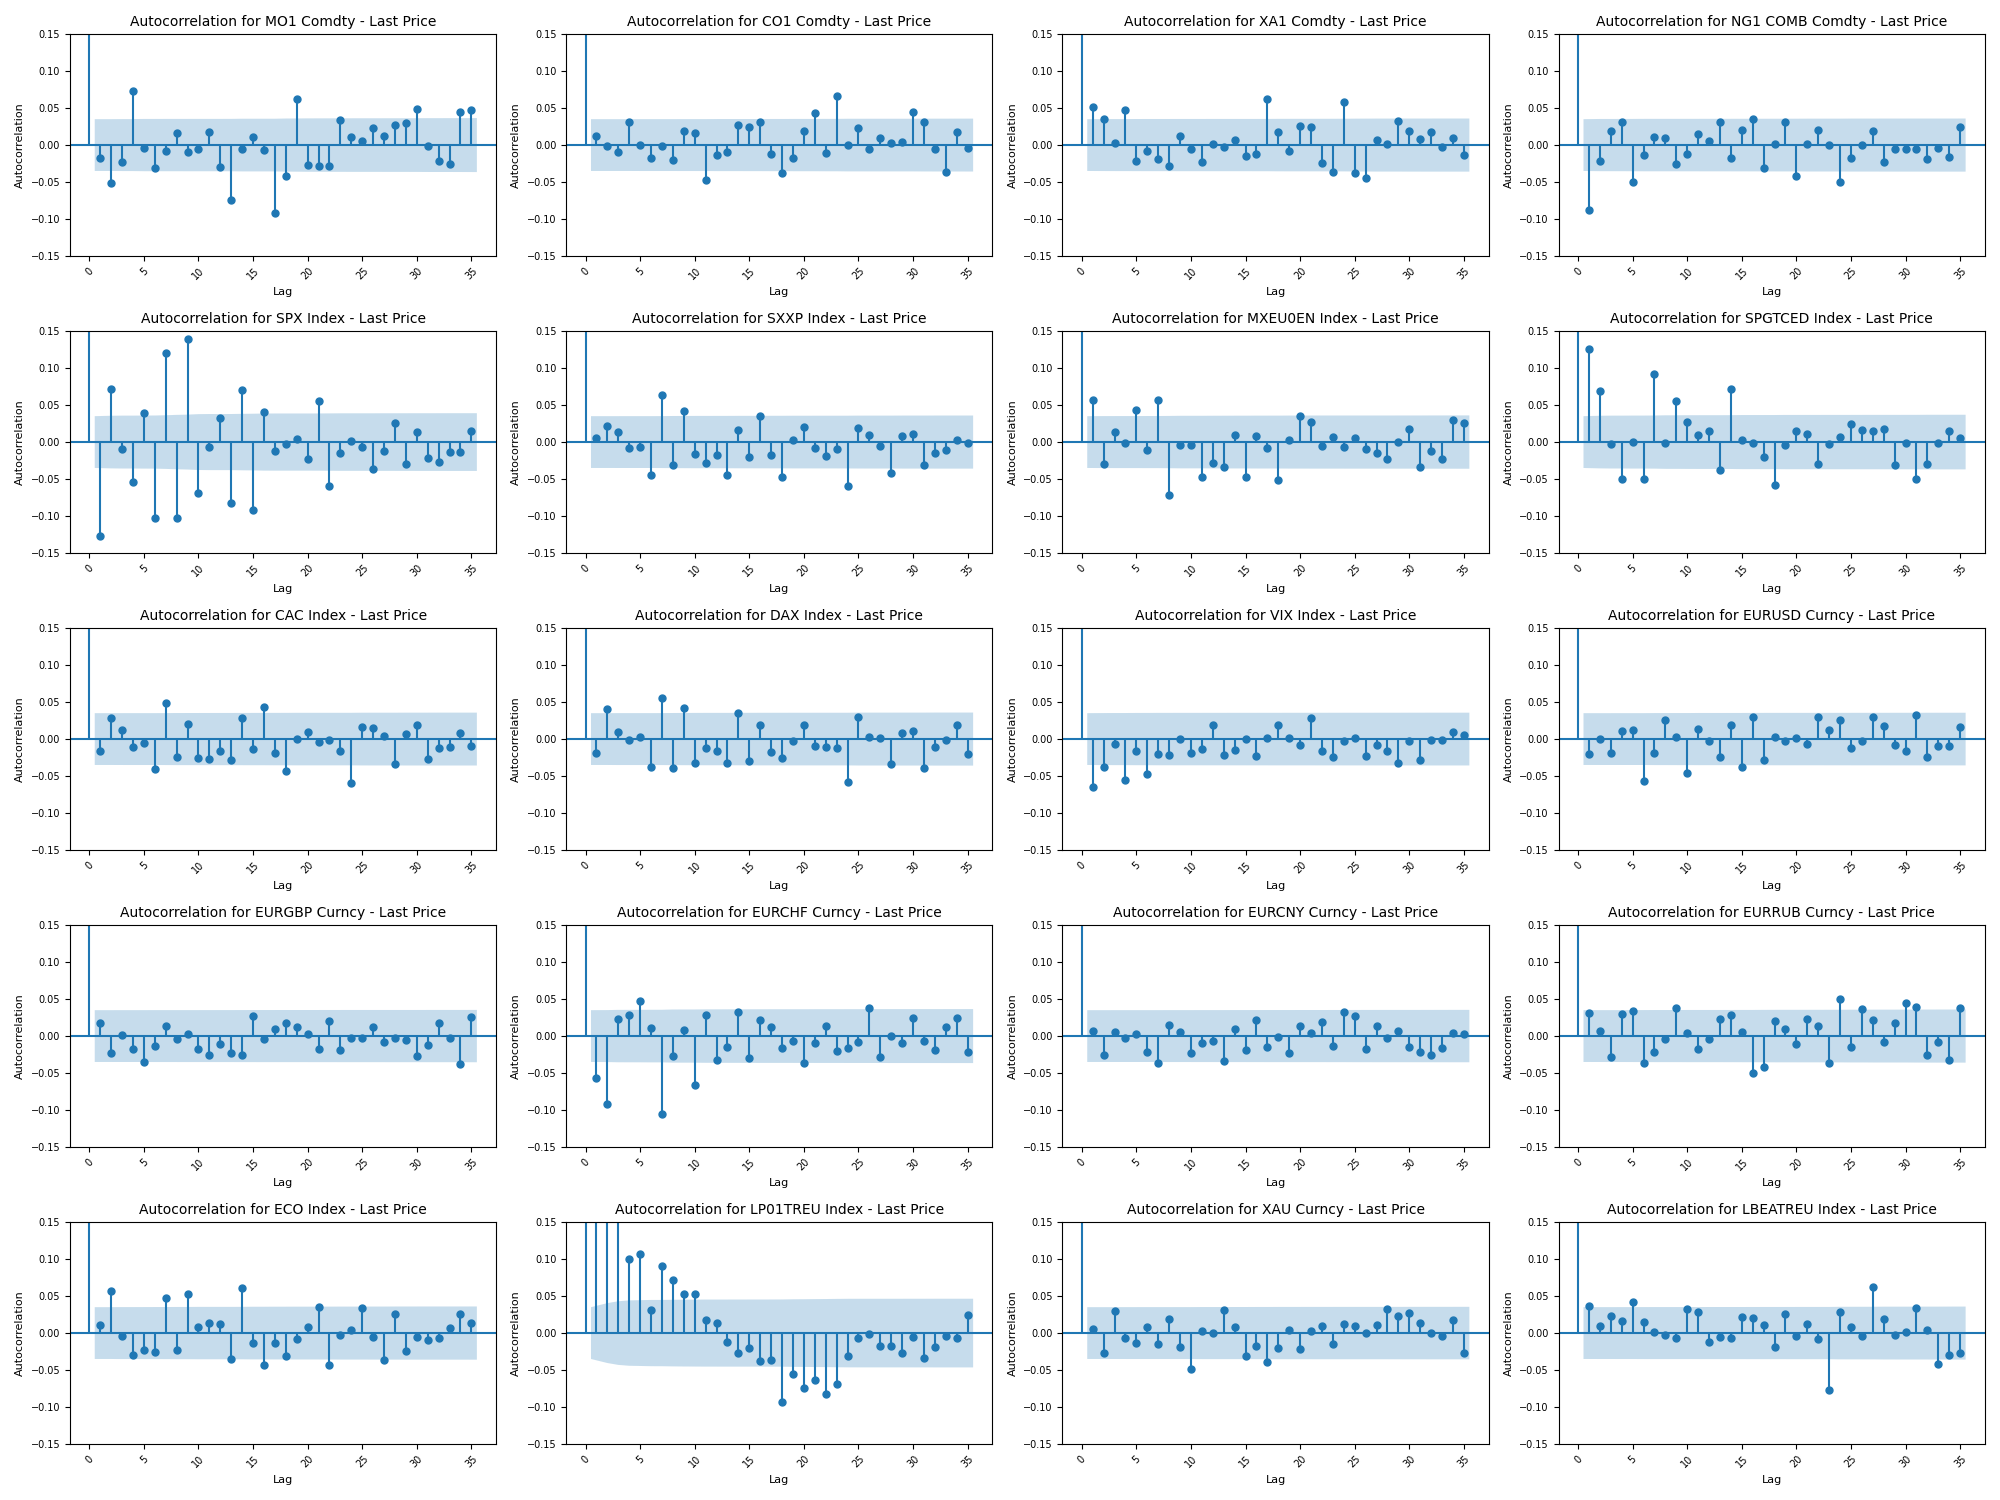
\includegraphics[width=1\textwidth]{graphics/acfplots.png}
\caption{ACF plots for each of the variables.}
\label{fig:acfplots}
\end{figure}

\begin{figure}[H]
\centering
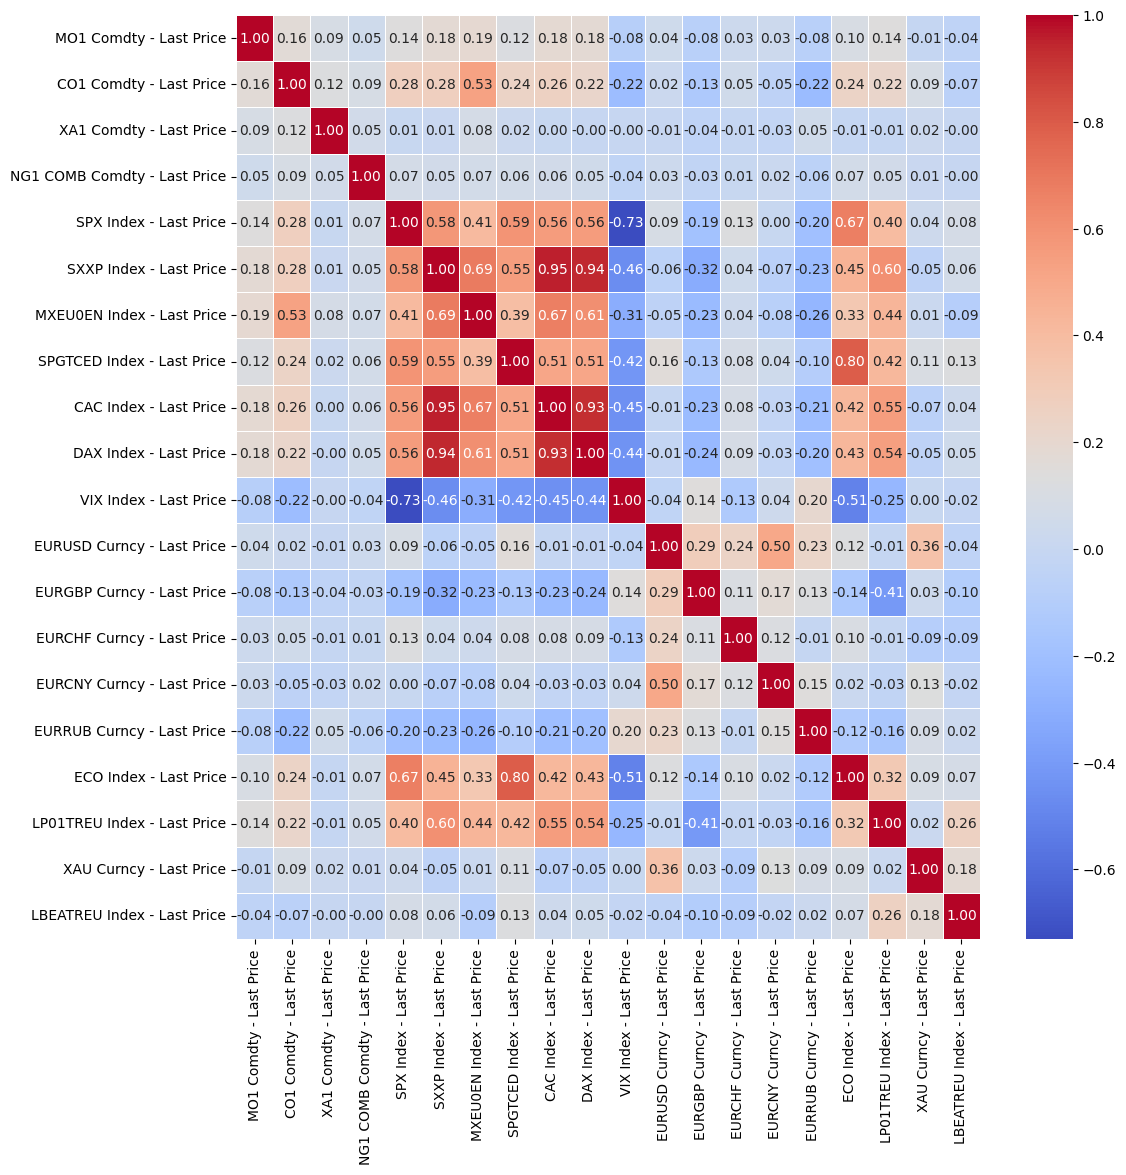
\includegraphics[width=1\textwidth]{graphics/corrtable2.png}
\caption{Correlation matrix of relevant features.}
\label{fig:correlationplot}
\end{figure}

\section{Appendix: Arch-Garch modelling discussion}
\label{appendix:archgarch}

The logarithm returns of each random variable are an input to this model and due to optimization difficulties with small numbers of less than one, which is the case with daily, financial logarithm returns, we scale all variables by a factor of 1000. For the non-dynamic Bayesian network, to search for the best performing AR-Garch models, we run a loop testing all possible values of $lag$, $p$ and $q$ in the ranges of 0 to 7 (incl.) for $lag$ and 1 to 9 (incl.) for the values of $p$ and $q$. Testing a variation of these values allows for fitting the model that presents the most accuracy with a minimum of the Bayesian Information Criteria (BIC) score possible. For the dynamic Bayesian network we consequently, set the AR mode to “Zero”, meaning no autoregressive mean model is present and run the same for loop for parameters $p$ and $q$ only. Such saved residuals are divided by a factor of 1000 to bring them down to their original scale for simplicity of further operations.

\begin{table}[H]
\centering
\small
\resizebox{\textwidth}{!}{
\begin{tabularx}{\textwidth}{|X|l|l|l|l|}
\hline
\textbf{Name} & \textbf{Lag} & \textbf{p} &  \textbf{q} & \textbf{BIC} \\
\hline
CAC Index & 1 & 1 & 1 & 23032.911114 \\
CO1 Comdty & 2 & 1 & 1 & 27151.131000 \\
DAX Index & 1 & 1 & 1 & 23183.164622 \\ 
ECO Index & 5 & 1 & 1 & 27178.144959 \\
EURCHF Curncy & 2 & 1 & 1 & 15248.167207 \\
EURCNY Curncy & 2 & 1 & 1 & 17737.700943 \\ 
EURGBP Curncy & 2 & 1 & 1 & 17817.950002 \\
EURRUB Curncy & 7 & 1 & 2 & 22699.691162 \\ 
EURUSD Curncy & 7 & 1 & 1 & 18264.746748 \\
LBEATREU Index & 0 & 1 & 1 & 13373.936223 \\ 
LP01TREU Index & 2 & 1 & 1 & 11344.578947 \\
MO1 Comdty & 7 & 1 & 1 & 29216.371639 \\ 
MXEU0EN Index & 3 & 1 & 2 & 24764.023812 \\
NG1 COMB Comdty & 7 & 1 & 1 & 30311.695942 \\ 
SPGTCED Index & 7 & 1 & 1 & 24417.201207 \\
SPX Index & 1 & 1 & 1 & 21854.044159 \\
SXXP Index & 0 & 1 & 1 & 21979.084816 \\
VIX Index & 7 & 1 & 1 & 35046.669846 \\
XA1 Comdty & 4 & 1 & 1 & 23832.359127 \\
XAU Curncy & 3 & 1 & 1 & 22174.697858 \\
\hline
\end{tabularx}
}
\caption{Best lag, p and q values, with minimum BIC per variable. Transformation for the non-dynamic Bayesian network.}
\label{tab:bngarch}
\end{table}

\begin{table}[H]
\centering
\small
\resizebox{\textwidth}{!}{
\begin{tabularx}{\textwidth}{|X|l|l|l|}
\hline
\textbf{Name} & \textbf{p} &  \textbf{q} & \textbf{BIC} \\
\hline
CAC Index & 1 & 1 & 23054.370236 \\
CO1 Comdty & 1 & 1 & 27147.702956 \\
DAX Index & 1 & 1 & 23207.687353 \\
ECO Index & 1 & 1 & 27187.836767 \\
EURCHF Curncy & 1 & 1 & 15256.103895 \\
EURCNY Curncy & 1 & 1 & 17733.174518 \\
EURGBP Curncy & 1 & 1 & 17813.439443 \\
EURRUB Curncy & 1 & 2 & 22701.914041 \\
EURUSD Curncy & 1 & 1 & 18266.720483 \\
LBEATREU Index & 1 & 1 & 13396.180696 \\
LP01TREU Index & 1 & 1 & 11859.606579 \\
MO1 Comdty & 1 & 1 & 29251.071332 \\
MXEU0EN Index & 1 & 1 & 24768.371503 \\
NG1 COMB Comdty & 1 & 1 & 30327.764376 \\
SPGTCED Index & 1 & 1 & 24482.172423 \\
SPX Index & 1 & 1 & 21915.317902 \\
SXXP Index & 1 & 1 & 22007.178318 \\
VIX Index & 1 & 1 & 35137.276338 \\
XA1 Comdty & 1 & 1 & 23855.780515 \\
XAU Curncy & 1 & 1 & 22173.202901 \\
\hline
\end{tabularx}
}
\caption{Best p and q values, with minimum BIC per variable. Transformation for the dynamic Bayesian network.}
\label{tab:dynamicbngarch}
\end{table}

\section{Appendix: Structure learning algorithm tests and graph evaluation}
\label{appendix:graphtests}

\begin{figure}[ht]
\centering
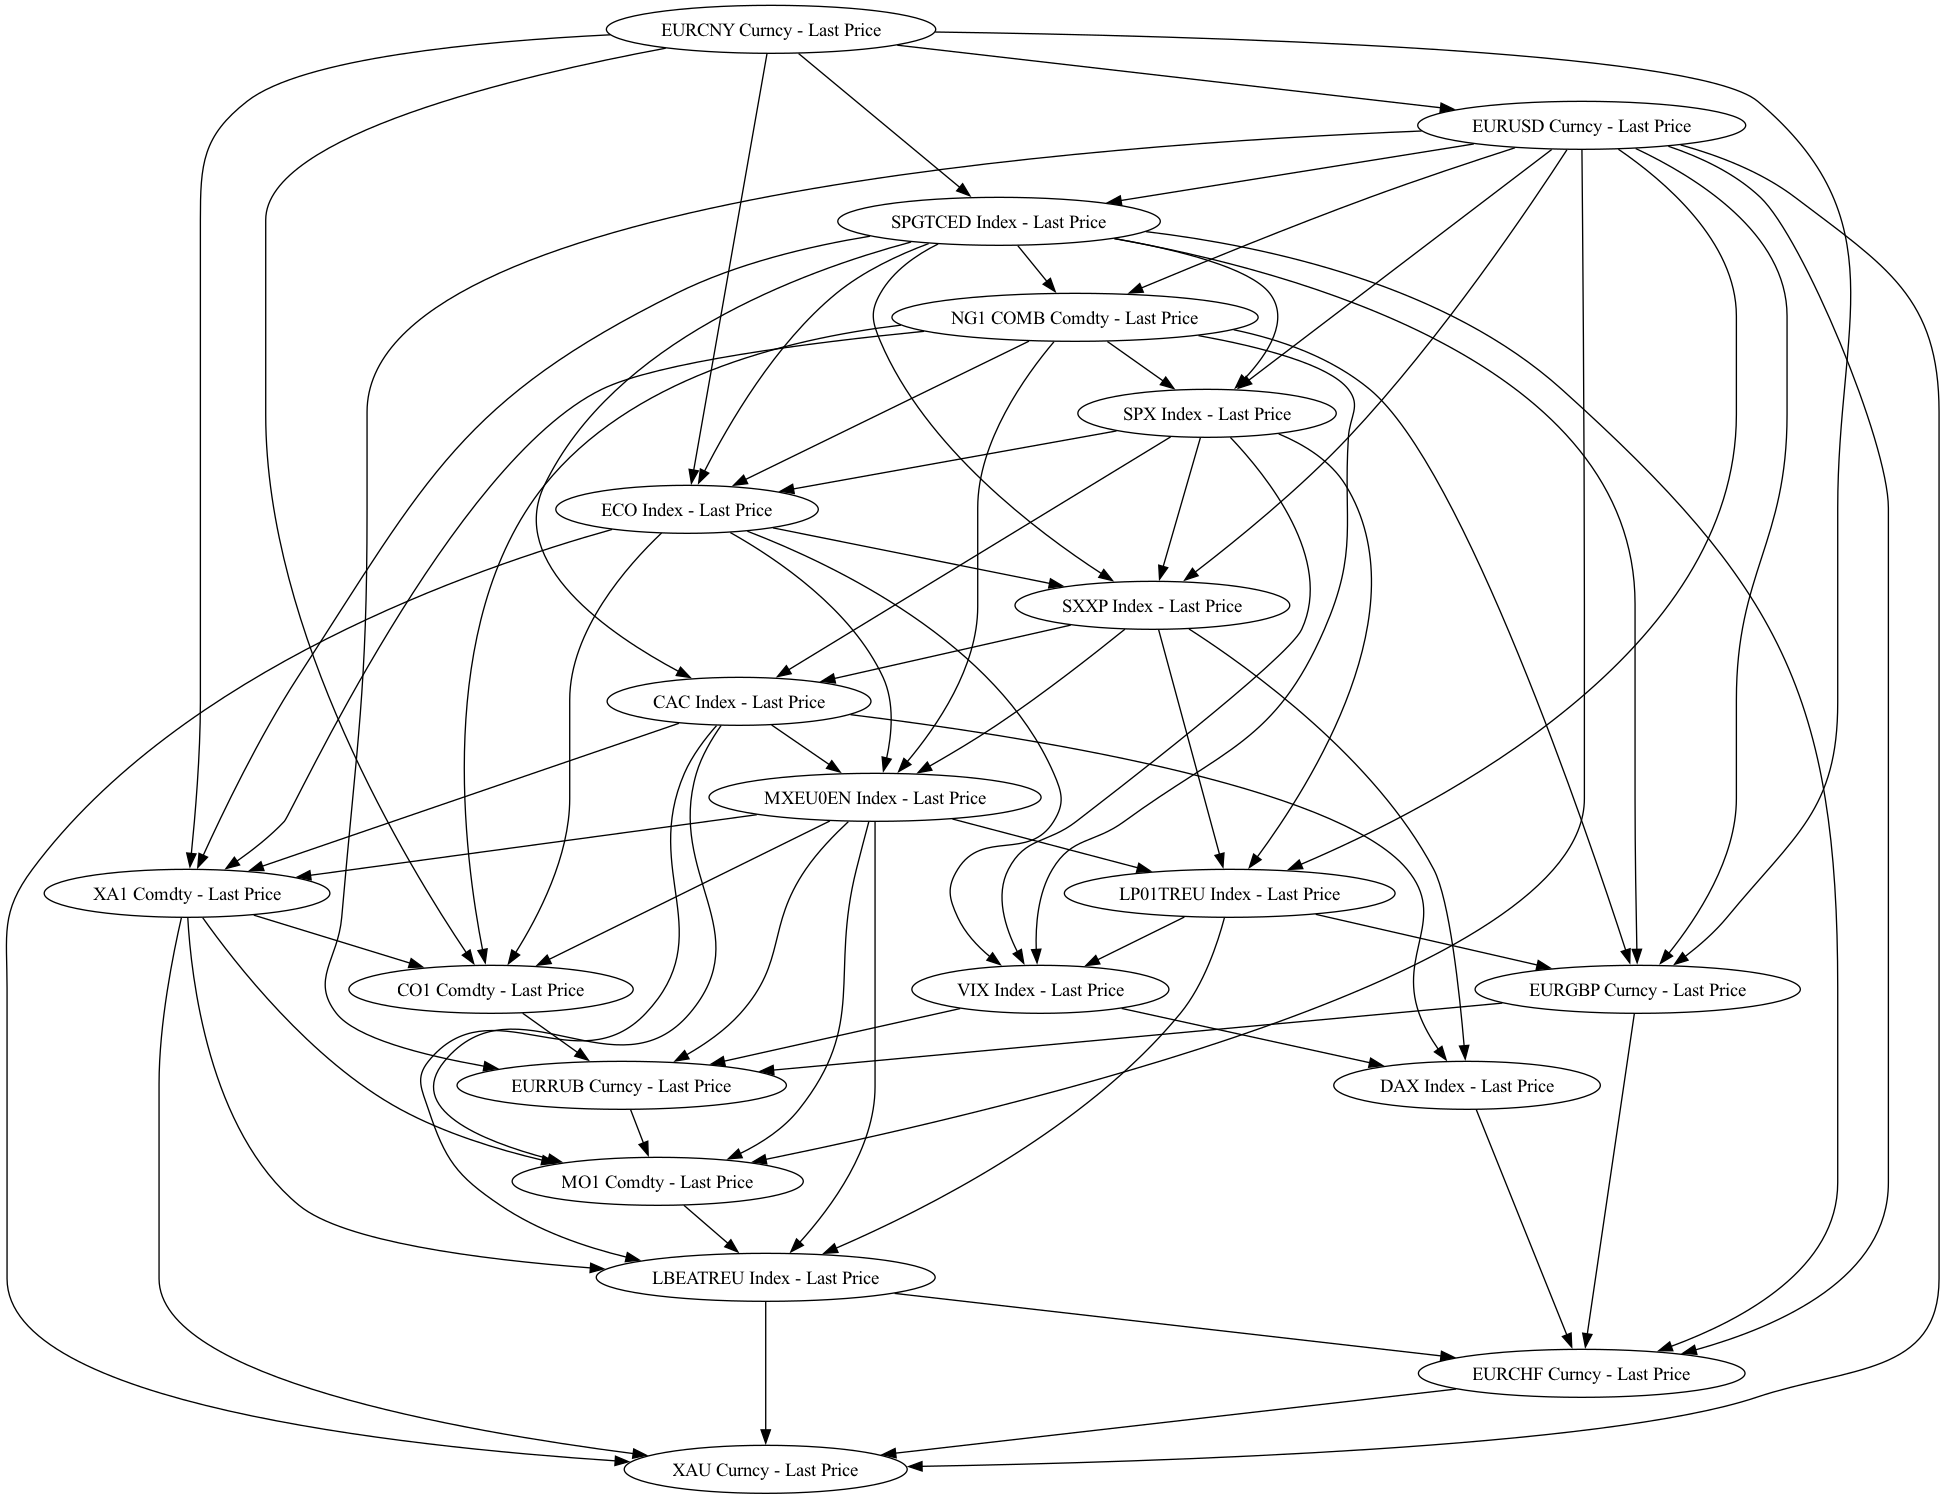
\includegraphics[width=\textwidth, keepaspectratio]{graphics/HCAICv3.png}
\caption{Graph structure derived using the Hill Climb algorithm with AIC as a score metric.}
\label{fig:netaic}
\end{figure}

\begin{figure}[ht]
\centering
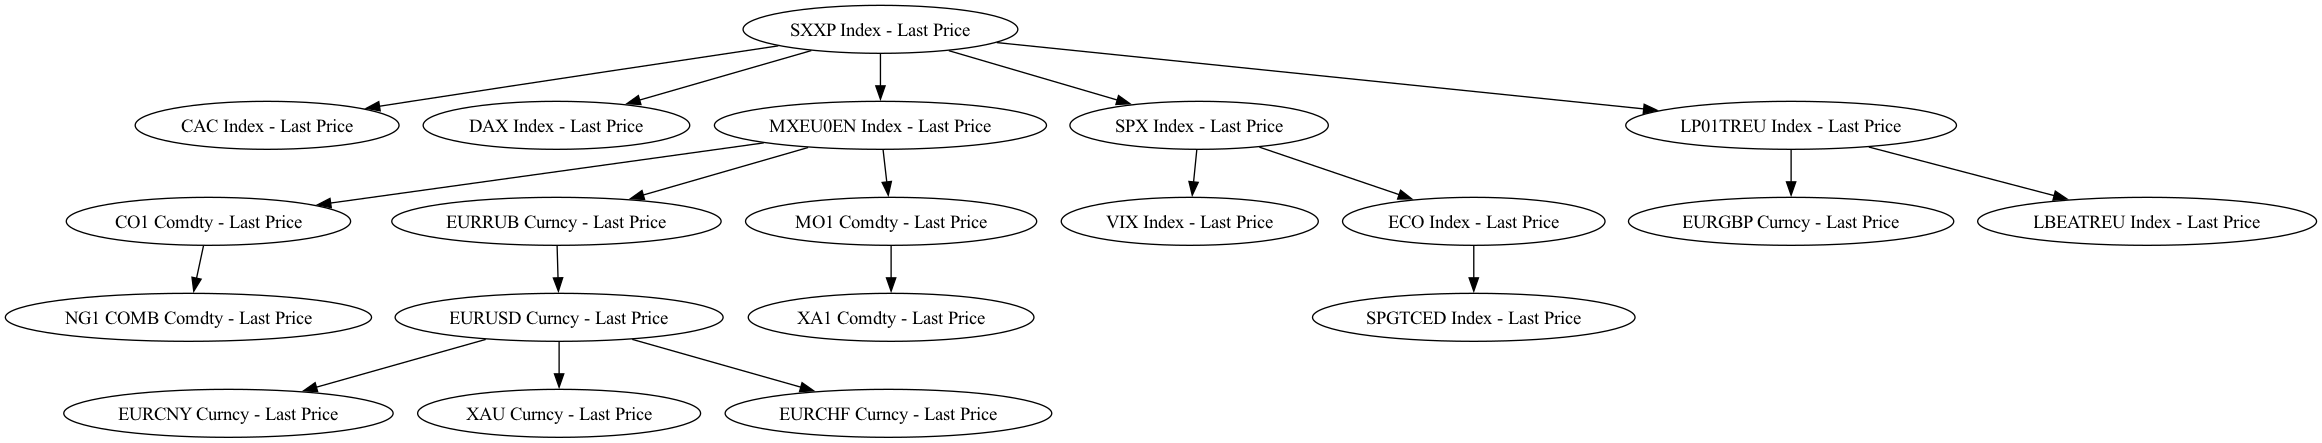
\includegraphics[width=1\textwidth]{graphics/TreeSChowLiu.png}
\caption{Graph structure derived using the Tree Search algorithm.}
\label{fig:nettreesearch}
\end{figure}

\begin{figure}[ht]
\centering
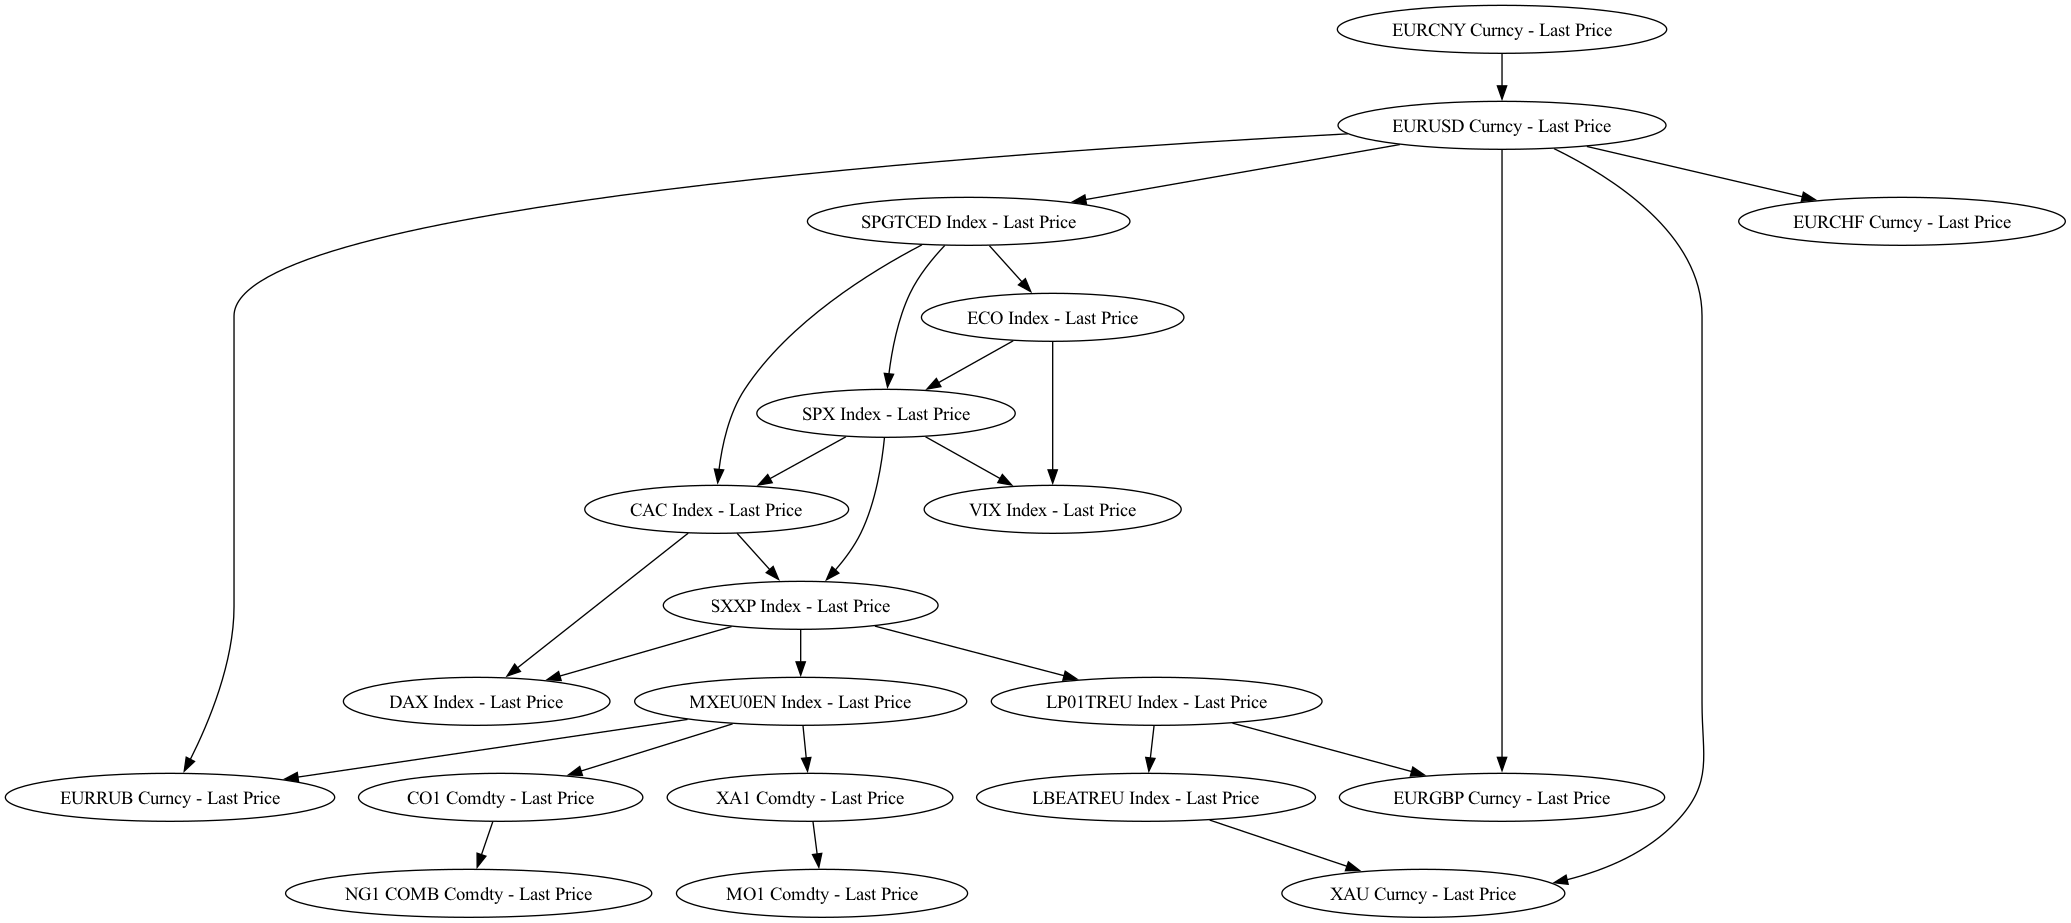
\includegraphics[width=1\textwidth]{graphics/HCBICTabu100v2.png}
\caption{Graph structure derived using the Hill Climb algorithm with BIC as a score metric.}
\label{fig:netbic}
\end{figure}

\begin{figure}[ht]
\centering
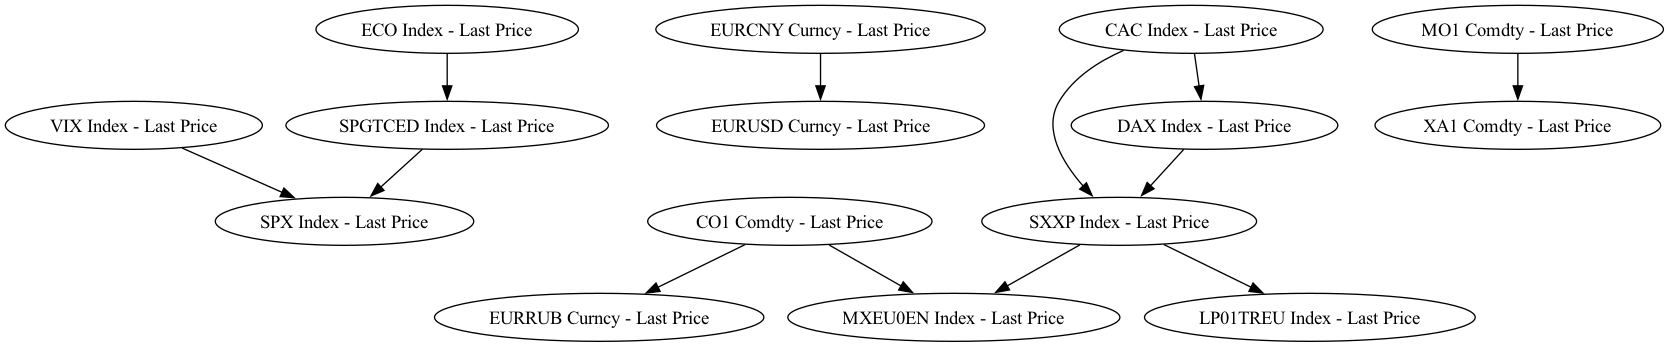
\includegraphics[width=1\textwidth]{graphics/PC.png}
\caption{Graph structure derived using the PC algorithm.}
\label{fig:netpc}
\end{figure}

\begin{figure}[ht]
\centering
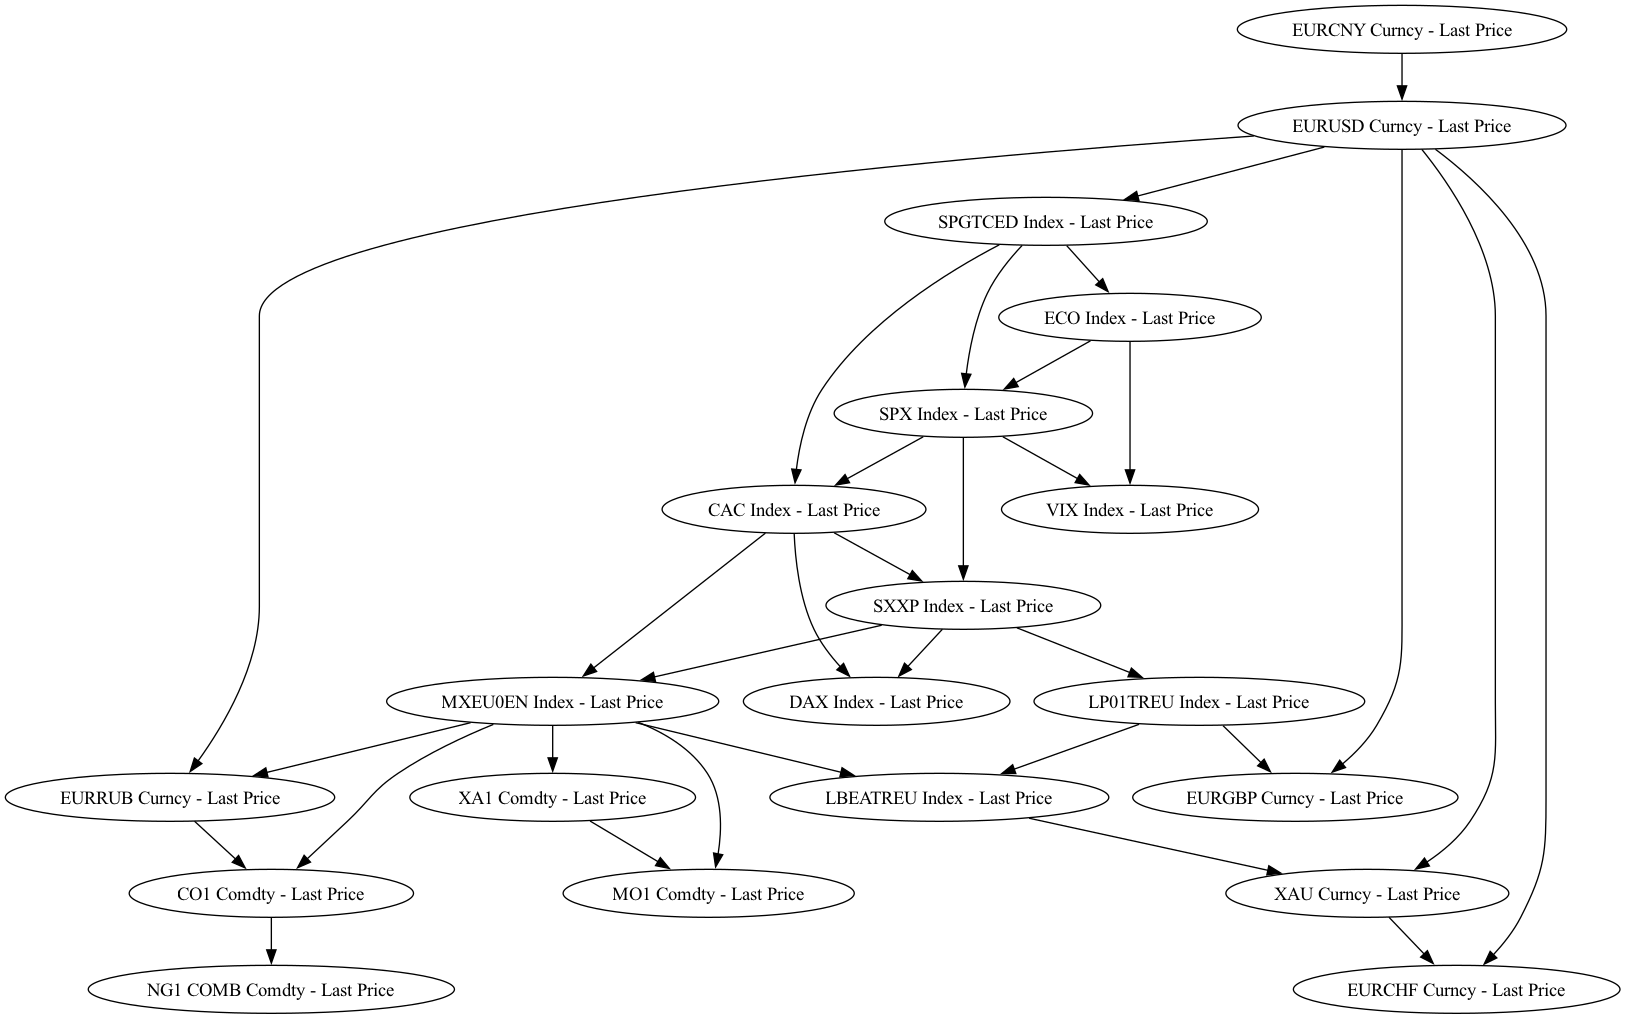
\includegraphics[width=1\textwidth]{graphics/HCBDeu10v5.png}
\caption{Our chosen BDeu network (Graphviz version).}
\label{fig:netbdeu}
\end{figure}

\end{document}
